\documentclass[a4paper,11pt]{article}
\pdfoutput=1 % if your are submitting a pdflatex (i.e.~if you have
% images in pdf, png or jpg format)

\usepackage{jheppub} % for details on the use of the package, please see the JHEP-author-manual

\addtolength{\textwidth}{1.0cm}      % widen text block
\addtolength{\oddsidemargin}{-0.5cm}
\addtolength{\evensidemargin}{-0.5cm}
\addtolength{\textheight}{1.5cm}     % more vertical space
\addtolength{\topmargin}{-0.75cm}

% Tighten spacing overrides
\linespread{0.96}
\setlength{\abovedisplayskip}{5pt}
\setlength{\belowdisplayskip}{5pt}

%\usepackage[utf8]{inputenc}

\usepackage{booktabs,multirow, quotes}

\usepackage[english]{babel}
\usepackage{amsthm,amsmath,amssymb,graphicx,xcolor,alltt}
\usepackage{framed}

%%%%%%%%%% Start TeXmacs macros
%\catcode`\<=\active \def<{
%\fontencoding{T1}\selectfont\symbol{60}\fontencoding{\encodingdefault}}
\newcommand{\longminus}{{-\!\!-}}
\newcommand{\tmop}[1]{\ensuremath{\operatorname{#1}}}


\newcommand{\beq}{\begin{equation}}
\newcommand{\eeq}{\end{equation}}
\newcommand{\bea}{\begin{eqnarray}}
\newcommand{\ea}{\end{eqnarray}}


\theoremstyle{remark}
\newtheorem{remark}{Remark}[section]
\newtheorem{example}{Example}[section]
\theoremstyle{theorem}
\newtheorem{lemma}{Lemma}[section]

%%%%%%%%%% End TeXmacs macros
\def\red{\color{red}}

\newcommand{\SR}[1]{{\red \bf [{SR:} #1]}}
\newcommand{\junchen}[1]{\textcolor{blue}{\textbf{[JR: #1]}}}
\def\cO{\mathcal{O}}

\makeatletter
\def\@fpheader{\ }
\makeatother

\title{Direct tests of conformal symmetry with Rydberg atoms: assessment and proposals}

 
\author{Junchen Rong$^1$,}
\author{Slava Rychkov$^2$}

% The "\note" macro will give a warning: "Ignoring empty anchor..."
% you can safely ignore it.

\affiliation{$^1$CPHT, CNRS, \'Ecole Polytechnique, Institut Polytechnique de Paris, Palaiseau, France\\
$^2$Institut des Hautes \'Etudes Scientifiques, 91440 Bures-sur-Yvette, France}


% e-mail addresses: one for each author, in the same order as the authors
\emailAdd{junchen.rong@polytechnique.edu}
\emailAdd{slava@ihes.fr}




\abstract{aaa}%This is a note on the measurement of 3pt function using Rydberg atom experiments.}



\begin{document} 
	
	\maketitle
	
	\flushbottom


\flushbottom

\section{Introduction}

Conformal invariance as a symmetry of critical fluctuations was first
conjectured by Polyakov in 1970 {\cite{Polyakov:1970xd}}. This idea was one of
the main motivations for the development of the conformal field theory (CFT),
by Polyakov and others {\cite{Polyakov:1974gs,Belavin:1984vu}}. By now it is
widely believed that a great majority of critical points---both thermodynamic
and quantum---possess an emergent conformal invariance, so that their
long-distance behavior is described by a CFT
{\cite{Cardy1987,Cardy:1996xt,tsvelik,giamarchi2003quantum,sachdev,fradkin}}.\footnote{Well-understood
	reasons {\cite{Polchinski:1987dy,Nakayama:2013is}} do allow rare exceptions
	--- critical points with only scale symmetry.} CFTs are tightly constrained
and can be solved, in low dimensions often exactly
{\cite{DiFrancesco:1997nk}}, while in higher dimensions approximately, using
the numerical conformal bootstrap {\cite{Poland:2018epd}}. Since the scaling
dimensions of CFT local operators are related to the critical exponents, which
can be experimentally measured, this provides many
\text{{\bfseries{indirect}}} tests of conformality,\footnote{We will use
	`conformal symmetry', `conformal invariance' and `conformality'
	interchangeably.} as reviewed e.g.~in {\cite{Henkel1999,Rychkov:2025zks}}. In
comparison, until recently little theoretical effort was devoted to designing
\text{{\bfseries{direct}}} tests {\cite{Pokrovskii1973,Gompper1985}}, and such
experiments were lacking {\cite{Rychkov:2025zks}}. For
\text{{\bfseries{thermodynamic}}} phase transitions, such tests are
challenging due to limitations of imaging with X-ray or neutron probes; see
{\cite{Podo:2026hfh}} for a recent proposal to use grazing scattering of
X-rays on critical binary alloys.

In the meantime, cold atom platforms {\cite{Browaeys:2020kzz,Morgado:2020jfo}}
revolutionized the experimental study of \text{{\bfseries{quantum}}} phase
transitions
{\cite{Bernien:2017ubn,Scholl:2020hzx,Ebadi:2020ldi,Semeghini:2021wls}}. Many
quantum Hamiltonians of interest can thus be engineered and their quantum
critical points can be studied
{\cite{Keesling:2018ish,Fang:2024uyf,Sun:2026aqf}}. These experiments can in
principle measure the state of every atom, providing a snapshot view of the
many-body wavefunction. Averaging over many snapshots allows to measure e.g.
the equal-time correlation functions
{\cite{Fang:2024uyf,Emperauger:2025raf}}---a classic way to probe conformality
{\cite{Polyakov:1970xd}}.

The time is therefore ripe for a general discussion of existing and future
tests of conformality in cold atom experiments, which will be our purpose
here. STOPPED HERE Our paper has two main parts. In Section \ref{sec:gen}, we
propose our view of which tests should count as indirect and which ones are
direct. Indirect tests are measurements of critical exponents, while direct
tests need to verify that correlation functions satisfy a conformal Ward
identity. We illustrate these points by examples of existing experiments.

Then, in Section \ref{sec:prop}, we discuss the simplest setups to test
conformality through measurements of equal-time two-point correlation
functions, with periodic and open boundary conditions. We present results of
our numerical simulations for experiments with 1D chains of Rydberg atoms. The
tests we imagine have not yet been performed due to limitations of decoherence
and/or insufficient adiabaticity of ground state preparation, but we hope they
are within reach. In Section \ref{sec:concl} we conclude.

Notation: D for spatial dimension, d for full spacetime dimension, as is
common in cond-mat and exp literature

\section{Tests of conformal invariance}\label{sec:gen}

\subsection{General discussion and the main direct test}

We find it convenient to divide possible experimental tests of conformality
into two groups - indirect and direct.

By means of analogy, suppose we have a 3D object and we wish to check its
rotational symmetry, i.e. if is it a round ball. A direct way would be to
stare at the object from different directions. An indirect way would be to
check the circumference to diameter ratio- does it equal $\pi$? Our point is
that symmetry is fundamentally about \text{{\bfseries{shapes}}} of objects. In
a quantum field theory the most basic object is a correlator. Hence, a direct
test of conformality should test constraints which it imposes on the
functional form of correlators. On the other hand, an indirect test can be a
measurement of a number predicted using techniques of CFT. Specific CFTs can
often be solved exactly, or numerically to very high accuracy. For example, an
infinite series of 2d CFTs called minimal models was solved exactly,
determining the local operator scaling dimensions and other properties
{\cite{Belavin:1984vu,DiFrancesco:1997nk}}. The main critical exponents
characterizing phase transitions can be expressed in terms of these scaling
dimensions {\cite{cardy1996scaling}}. Any measurement of a critical experiment
in agreement with a CFT prediction is an indirect test of conformality. Many
such indirect tests can be extracted from the literature
{\cite{Henkel1999,Rychkov:2025zks}}, even though the original experimental
papers may not have emphasized the connection with conformality.

Talking about CFT correlators, we should specify the geometry, including the
signature: Euclidean or Lorentzian. Euclidean signature is relevant for the
dscription of thermodynamic phase transitions, and Lorentzian signature for
the quantum ones. As a representative example, consider the $\mathcal{M} (3,
4)$ minimal model, also called 2d Ising CFT, since it describes the
universality class of the Ising phase transition. This theory has local
primary operators $\sigma, \epsilon$ of scaling dimensions $\Delta_{\sigma} =
1 / 8$, $\Delta_{\epsilon} = 1$. In infinite flat 2d space, the simplest
nontrivial correlators are two-point (2pt) and three-point (3pt) functions of
these primary operators:

\begin{align}
	\langle \mathcal{O}(x_1)\mathcal{O}(x_2) \rangle_{\mathbb{R}^2} & =
	\frac{1}{x_{12}^{2 \Delta_{\mathcal{O}}}}  \qquad (\mathcal{O}= \sigma,
	\epsilon) \hspace{0.17em},  \label{eq:two-point}\\
	\langle \sigma (x_1) \sigma (x_2) \epsilon (x_3) \rangle_{\mathbb{R}^2} & =
	\frac{C_{\sigma \sigma \epsilon}}{x_{12}^{2 \Delta_{\sigma} -
			\Delta_{\epsilon}} x_{31}^{\Delta_{\epsilon}} x_{32}^{\Delta_{\epsilon}}}
	\hspace{0.17em}, \quad C_{\sigma \sigma \epsilon} = 1 / 2. 
	\label{eq:three-point}
\end{align}

These formulas are valid in both signatures, interpreting $x^2_{ij}$ as either
Euclidean or Lorentzian distance squared between $x_i$ and $x_j$.\footnote{In
	the latter case, the distances are computed with infinitesimal imaginary parts
	for time differences, depending on the operator ordering, giving phases for
	light-like point separations. See e.g. {\cite{Hofman:2008ar}}.}

Which direct and indirect tests of conformality can be done in principle using
these formulas?

A direct test would be to measure the 3pt function \eqref{eq:three-point} and
see the given specific functional form in terms of just three parameters
$\Delta_{\sigma}, \Delta_{\epsilon}, C_{\sigma \sigma \epsilon}$. Indeed this
dependence was one of the earliest nontrivial predictions of conformal
symmetry {\cite{Polyakov:1970xd}}, obtained from covariance under conformal
maps, while scale symmetry alone would allow an infinite number of
possibilities {\cite{Rychkov:2016iqz}}. Measurements of infinite-volume 3pt
functions are complicated, and they were never attempted.\footnote{We thank
	Thomas Chalopin and David Cl{\'e}ment for a discussion of the possibility of
	realizing such a measurement in their experimental cold-atom platform
	{\cite{Allemand:2025pdq}}.} See Fig.~\ref{fig:flat}.

On the other hand, to measure the 2pt functions \eqref{eq:two-point} and see a
powerlaw would not be a direct test of conformality, but rather of the more
mundane scale symmetry.\footnote{2pt functions of primaries of unequal
	dimensions vanish by conformality {\cite{Polyakov:1970xd}}, but it's unclear
	how to test this experimentally. See {\cite{Podo:2026hfh}} for a critique of
	an early proposal by Pokrovsky
	{\cite{Pokrovskii1973,PatashinskiPokrovsky1979}}.}

Finally, one could use \eqref{eq:two-point} or \eqref{eq:three-point} to
measure $\Delta_{\sigma}$, $\Delta_{\epsilon}$, or $C_{\sigma \sigma
	\epsilon}$ in agreement with their exact CFT values. This would be an indirect
test.

\begin{figure}[h]\centering
	\begin{center}
		\resizebox{200pt}{!}{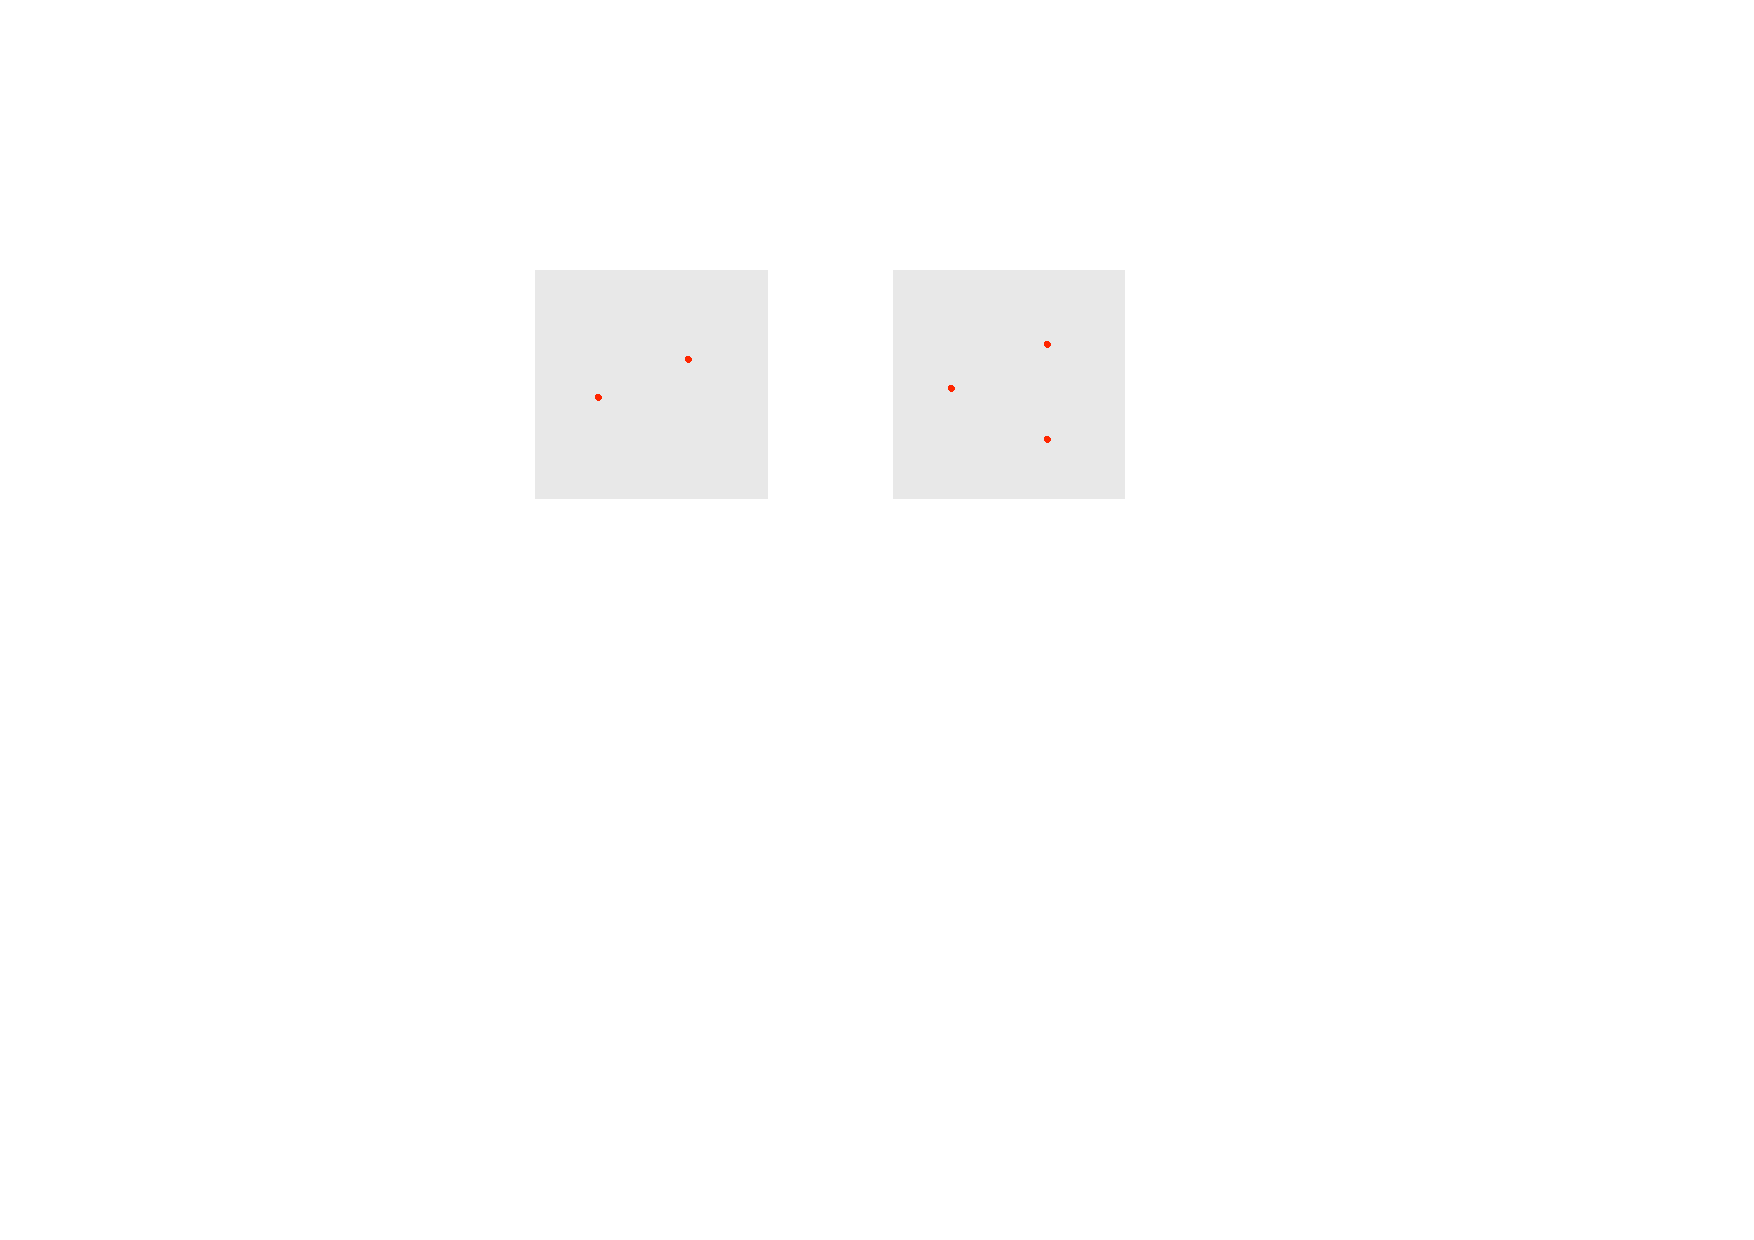
\includegraphics{fig-flat.pdf}}\label{fig:flat} 
	\end{center}
	\caption{Direct tests in infinite space: 2pt functions (left) test but scale
		symmetry, while 3pt functions (right) do test comformality but are hard to
		measure.}
\end{figure}

Let us now move to the finite volume case. Rydberg atom experiments are
typically done on groups of 20-200 atoms grouped in a 1D or 2D array. So for
us the finite volume case will be the most relevant. We will be comparing with
2d CFT, so we consider the 1D setup. The most convenient case is that of
periodic boundary conditions, when a chain of Rydberg atoms is arranged
periodically on a circle. We will also comment on the open boundary condition
case, when Rydberg atoms are arranged on an interval.

Let us assume that the chain of Rybberg atoms finds itself in the ground
state, with interactions tuned to be at the quantum critical point. How to get
such a state efficiently via adiabatic evolution will be discussed below. The
corresponding CFT geometry is the surface of a cylinder, where time runs
vertically, and constant time circular sections represent space where the
Rydberg atoms are positioned, Fig. \ref{fig:cyl}.

\begin{figure}[h]\centering
	\begin{center}
		\resizebox{200pt}{!}{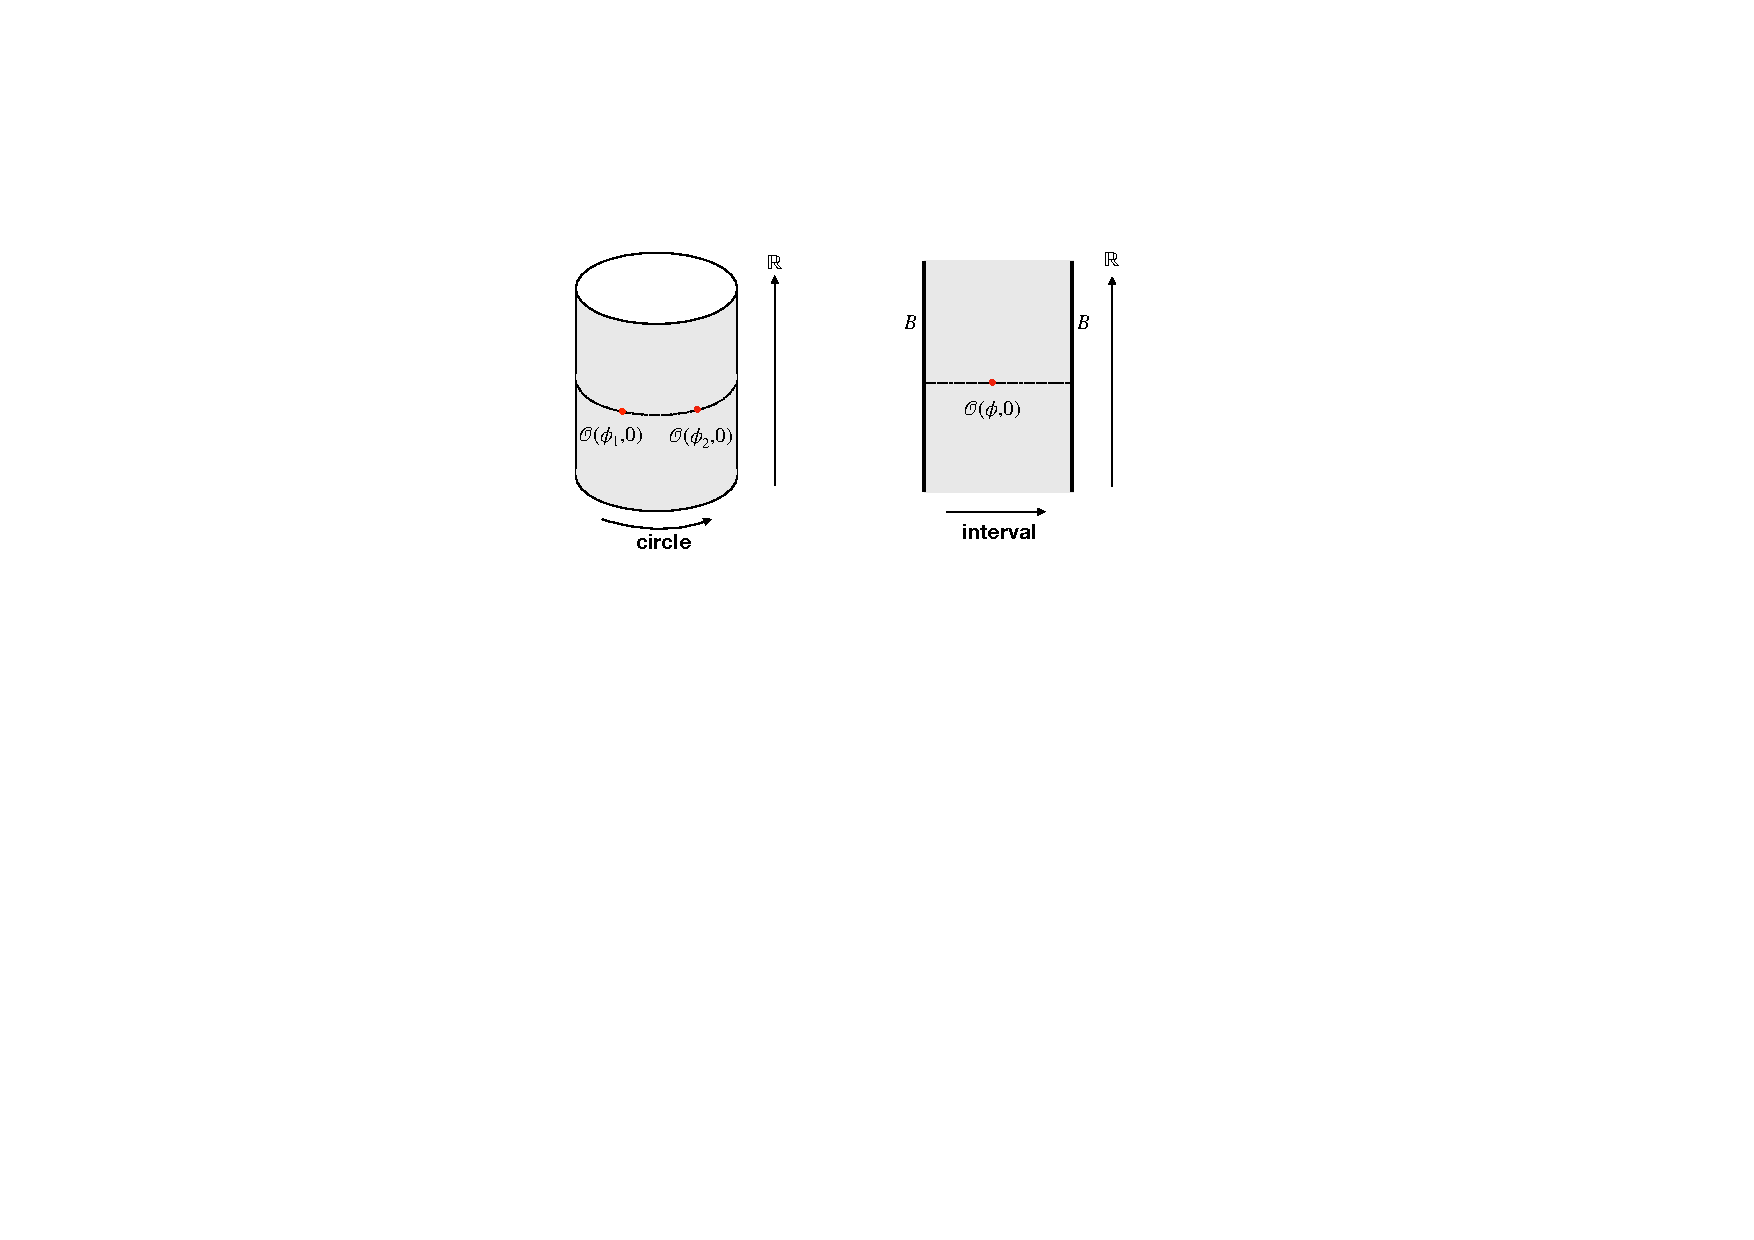
\includegraphics{fig-cyl.pdf}}\label{fig:cyl} 
	\end{center}
	\caption{A direct test of conformality in finite volume, using the equal
		time CFT 2pt function on the cylinder $S^1 \times \mathbb{R}$.
		{\color{red}{REMOVE: Right: 1pt function on the strip $[0, \pi] \times
				\mathbb{R}$ with identical boundary conditions. Remove also the right part
				of the figure.}}}
\end{figure}

Now it turns out that such a 1D finite-volume setup carries a theoretical
advantage for direct tests of conformality. We have seen that 2pt functions in
infinite volume would not test conformality but scale symmetry, and one would
have to go to 3pt functions in infinite-volume. But in finite circular volume
already 2pt functions test conformality! Indeed, while the scale symmetry is
broken by finite volume, conformality survives. In fact conformal group for
the 2d cylinder (or on any geometry which is, like the cylinder, equivalent to
the plane by a Weyl transformation) is as large as the conformal group of the
plane. This leads to constraints on correlators, which are nontrivial already
for 2pt functions. The 2pt function of a primary operator on the cylinder of
circumference $2 \pi$ is given by {\cite{Luscher:1974ez}}:
\begin{equation}
	\label{eq:2ptcyl} \langle \mathcal{O}(\phi_1, \tau_1)\mathcal{O}(\phi_2,
	\tau_2) \rangle_{\ensuremath{\operatorname{cyl}}} = \frac{1}{|2 \cosh
		(\tau_1 - \tau_2) - 2 \cos (\phi_1 - \phi_2) |^{\Delta_{\mathcal{O}}}}
	\hspace{0.17em},
\end{equation}
where $\phi_i \in [0, 2 \pi]$, $\tau_i \in \mathbb{R}$. We wrote this formula
for the Euclidean cylinder, while for the Lorentzian cylinder one has to do
the Wick rotation.

The salient features of Eq. \eqref{eq:2ptcyl} are: time-translation
invariance, and exponential decay at large Euclidean time separation $\tau_1 -
\tau_2$.

To find Eq. \eqref{eq:2ptcyl}, the easiest is to use the above-mentioned Weyl
equivalence of the cylinder and the plane, realized by the exponential map.
Thus \eqref{eq:2ptcyl} can be easily obtained from the infinite-plane result
\eqref{eq:two-point} {\cite{DiFrancesco:1997nk}}. However, we stress that one
can in principle also derive Eq. \eqref{eq:2ptcyl} without using the
Weyl-equivalence, by staying on the cylinder and using the conformal group of
the cylinder.

For the Hamiltonian dynamics in real time, like in the Rydberg atom
experiments, one needs to Wick-rotate \eqref{eq:2ptcyl} to Lorentzian
signature. Then the 2pt function exhibits oscillating behavior in the time
direction {\cite{Luscher:1974ez}}. We don't show the full formula here,
because below we will focus on the equal time case, in which case the 2pt
function reduces to
\begin{equation}
	\label{eq:2ptcylequal} \langle \mathcal{O}(\phi_1, 0)\mathcal{O}(\phi_2, 0)
	\rangle_{\ensuremath{\operatorname{cyl}}} = \frac{1}{|2 \sin \frac{\phi_1 -
			\phi_2}{2} |^{2 \Delta_{\mathcal{O}}}},
\end{equation}
for both the Euclidean and Lorentzian signature.

We see that the functional form of the finite-volume correlator
\eqref{eq:2ptcylequal} is fixed at all distances, including distances of the
order of the size of the spatial manifold, in terms of just one parameter
$\Delta_{\mathcal{O}}$. While this is well known, we would like to stress here
that this is a direct consequence of conformality. Therefore, to see this
functional form experimentally would be a direct test of conformality.

\subsection{Other direct tests}

Below we will mostly focus on the possibility of a direct test of Eq.
\eqref{eq:2ptcylequal}. But in this section we will briefly discuss two other
possible direct tests.

\text{{\bfseries{I.}}} Instead of periodic boundary conditions (circle), one
may choose to position Rydberg atoms on an interval. Then, the relevant CFT
geometry is the strip, Fig. \ref{fig:strip}. There is some freedom for the
boundary conditions on the two sides of the strip, playing with interactions
of Rydberg atoms close to the endpoints. At the critical point, the effect of
boundary conditions is described by conformal boundary conditions $B_1$ and
$B_2$ on the two boundaries. In this strip setup, already 1pt functions can
test conformal symmetry directly. In the simplest case with equal boundary
conditions, $B_1 = B_2$, the 1pt function of a primary operator on the strip
of width $\pi$ takes the form:
\begin{equation}
	\label{eq:1ptstrip} \langle \mathcal{O}(\phi, 0)
	\rangle_{\ensuremath{\operatorname{strip}}} = \frac{A_{\mathcal{O}}}{(2 \sin
		\phi)^{\Delta_{\mathcal{O}}}} \hspace{0.17em}, \quad 0 < \phi < \pi
	\hspace{0.17em} \quad (B_1 = B_2) \hspace{0.17em} .
\end{equation}
This is usually shown by conformal-transforming the upper-half-plane 1pt
function $\langle \mathcal{O}(z) \rangle_{\ensuremath{\operatorname{UHP}}} =
A_{\mathcal{O}} / (2 \hspace{0.17em} \text{Im} z)^{\Delta_{\mathcal{O}}}$
{\cite{Cardy:1984bb}} to the strip {\cite{Calabrese:2006rx}}. But this can
also be in principle derived by staying on the strip.

\begin{figure}[h]\centering
	\begin{center}
		\resizebox{200pt}{!}{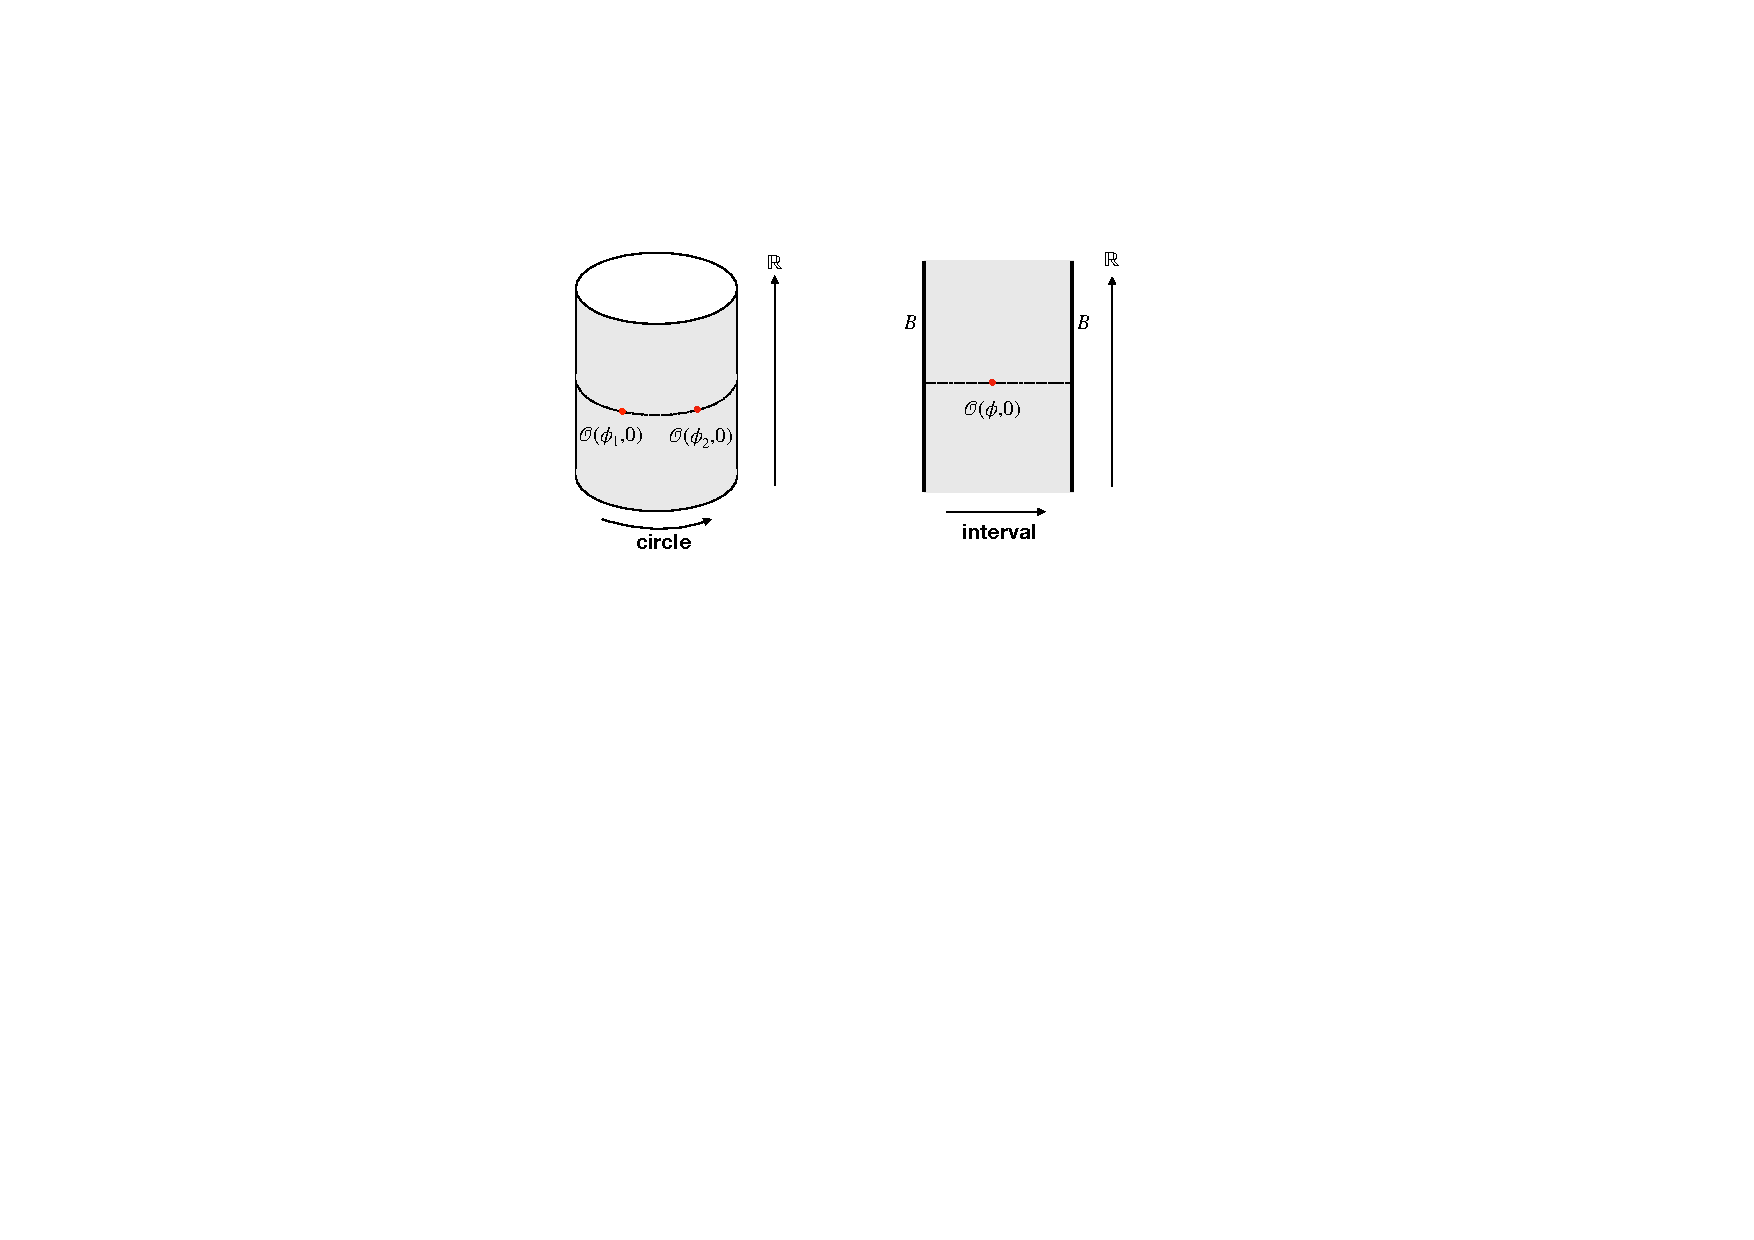
\includegraphics{fig-cyl.pdf}}\label{fig:strip} 
	\end{center}
	\caption{A direct test of conformality in finite volume, using the CFT 1pt
		function on the strip $[0, \pi] \times \mathbb{R}$. {\color{red}{REMOVE: the
				left part of the figure.}}}
\end{figure}

For a nontrivial test, $A_{\mathcal{O}}$ in \eqref{eq:1ptstrip} should not be
zero, which may happen due to global symmetry reasons. For example, for
$\mathcal{O}= \sigma$ in the 2d Ising CFT, the boundary condition should break
global $\mathbb{Z}_2$ for $A_{\mathcal{O}}$ to be nonzero, hence it should be
either ``spin-up'' or ``spin-down'' boundary condition $| + \rangle$, $| -
\rangle$ and not the ``free'' boundary condition $|f \rangle$.

What is easier: testing 1pt function \eqref{eq:1ptstrip} or testing 2pt
function \eqref{eq:2ptcylequal}? Our investigations suggest that testing
\eqref{eq:2ptcylequal} is easier. A significant advantage of
\eqref{eq:2ptcylequal} is translation invariance. It helps in the measurement,
since averaging over translations improves statistics. It also helps during
the adiabatic evolution when preparing the ground state, since the whole
adiabatic evolution takes place in the translationally invariant subsector of
the Hilbert space. Eq. \eqref{eq:1ptstrip} has no comparable advantages.
Moreover, in our numerical experiments, \eqref{eq:1ptstrip} was affected by
large corrections to scaling near the boundaries.\footnote{One can phrase this
	by saying that there is an ambiguity where the ``true'' CFT boundary is
	located compared to the Rydberg chain boundary.} For these reasons below we
will focus on the possible tests of \eqref{eq:2ptcylequal} and we will not
report any results for \eqref{eq:1ptstrip}.

\text{{\bfseries{II.}}} Another possible test of conformality would be to test
the operator-state correspondence (OSC), which can be tested both on the
cylinder and on the strip.

Consider the list $\{ \mathcal{O}_n \}_{n = 0}^{\infty}$ of all local
operators of a CFT, both primaries and their descendants. The OSC on the
cylinder says that:
\begin{itemize}
	\renewcommand{\labelitemi}{$\bullet$}\renewcommand{\labelitemii}{$\bullet$}\renewcommand{\labelitemiii}{$\bullet$}\renewcommand{\labelitemiv}{$\bullet$}\item
	such operators are in one-to-one correspondence with the energy eigenstates
	$| n \rangle$ on the circle, with the identity operator $\mathcal{O}_0$
	corresponding to the ground state $| 0 \rangle$;
	
	\item scaling dimensions $\Delta_{\mathcal{O}_n}$ and the gaps $E_n - E_0$
	above the ground state are proportional to each other.
\end{itemize}
The proportionality factor involves the ``speed of light'' of the emergent
Lorentz invariance, as well as the physical length of space. To eliminate
these factors, it is convenient to study the energy gap ratios. Then the OSC
predicts that
\begin{equation}
	\label{eq:ratio-rel} (E_n - E_0) / (E_m - E_0) = \Delta_{\mathcal{O}_n} /
	\Delta_{\mathcal{O}_m} \hspace{0.17em} \quad \text{(cylinder)} .
\end{equation}
There is also a variant of OSC for the strip with boundary conditions $B_1$
and $B_2$. There, there is correspondence between boundary (or
boundary-changing if $B_1 \ne B_2$) CFT operators $\hat{\mathcal{O}}_n$ on the
one hand, and states on the interval on the other hand. There is also a
relation analogous to \eqref{eq:ratio-rel} with $\Delta_{\mathcal{O}_n} \to
\Delta_{\hat{\mathcal{O}}_n}$. {\color{red}{ADD REFS}}

The OSC is a fundamental property of CFT. Its origin can be traced to the
already mentioned fact that the cylinder is Weyl-equivalent to the plane,
while the strip to the half-plane (see Fig.~\ref{fig:OSC}). Therefore, a test
of relation \eqref{eq:ratio-rel} would also qualify as a direct test of
conformality.\footnote{We thank the authors of {\cite{Wang:2026prw}} for a
	discussion.}

\begin{figure}[h]\centering
	\begin{center}
		\resizebox{200pt}{!}{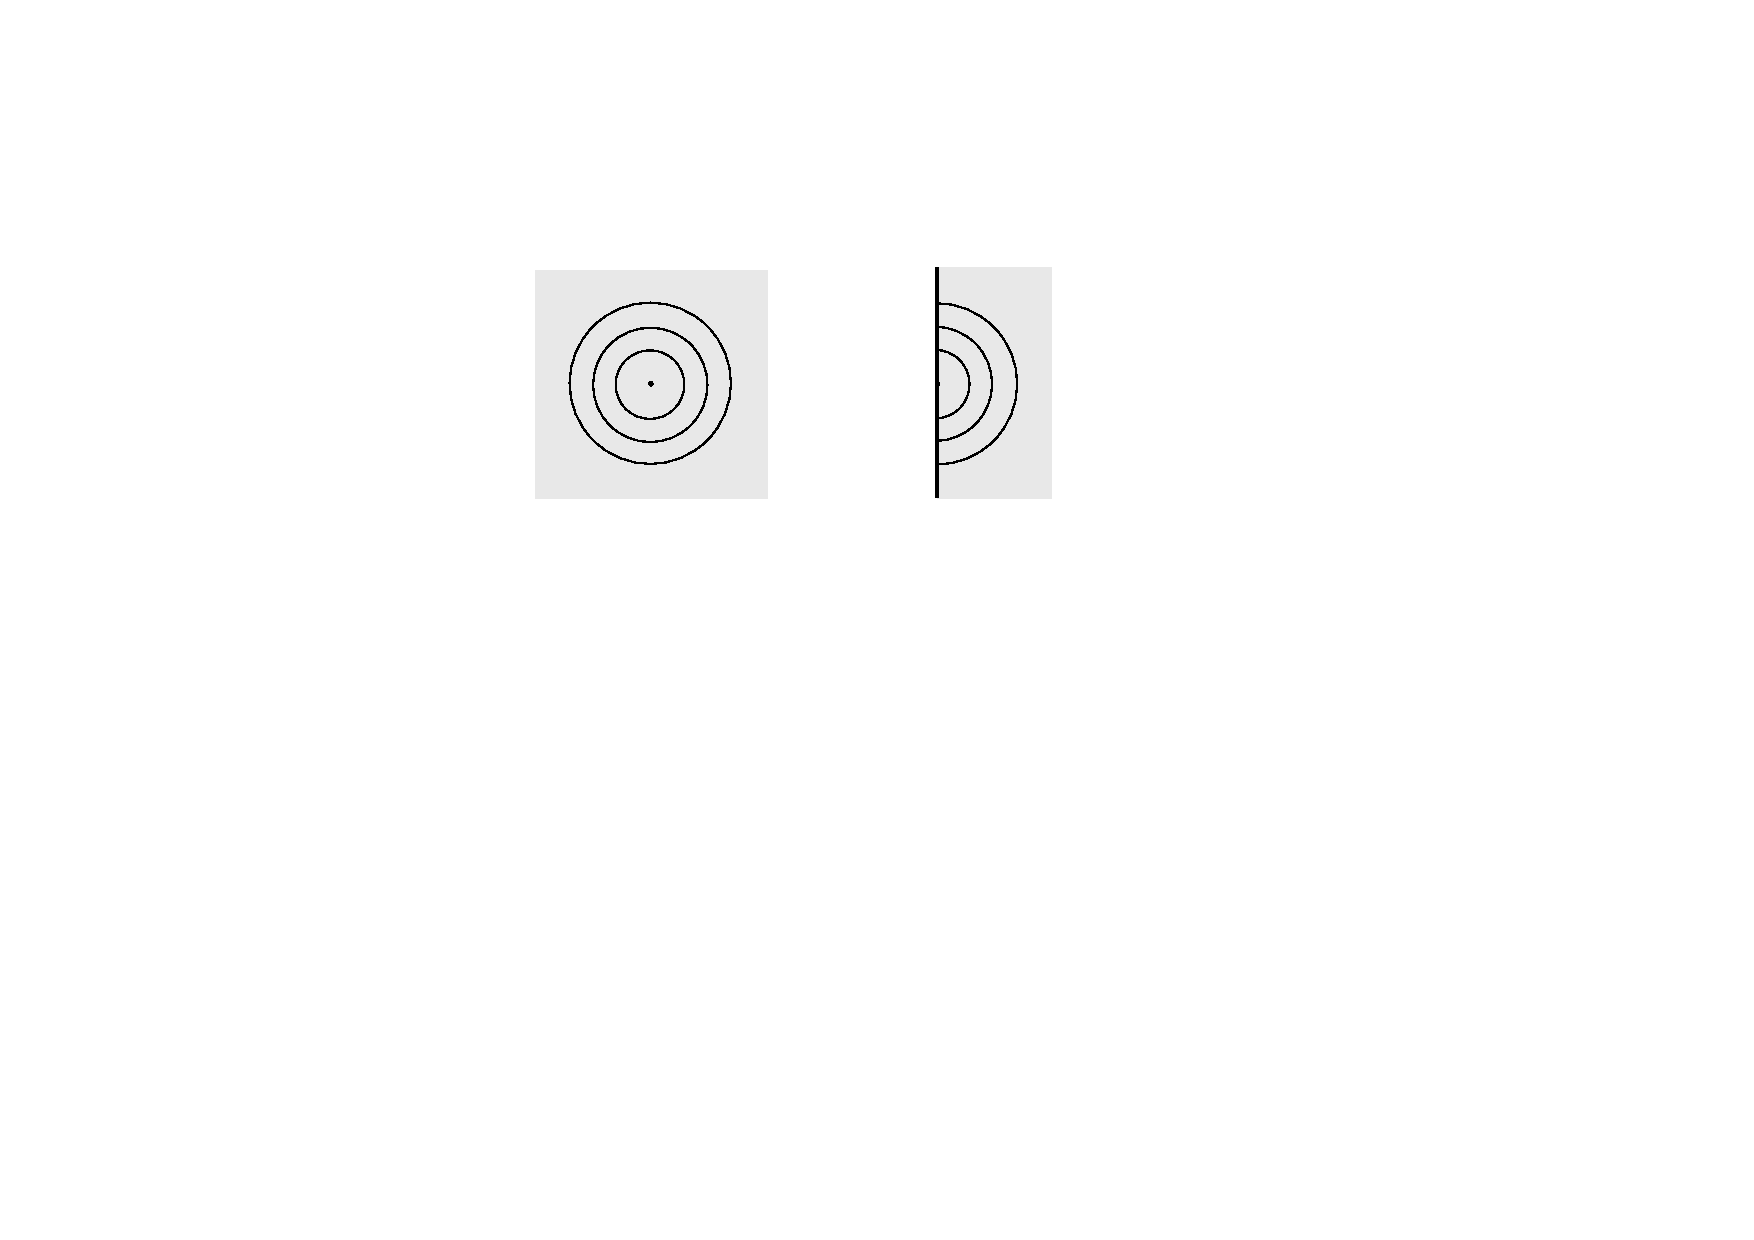
\includegraphics{fig-OSC.pdf}}\label{fig:OSC} 
	\end{center}
	\caption{Justification of OSC. Cylinder, resp. strip, can be conformally
		mapped onto the plane (left), resp. half-plane (right), with constant time
		sections mapped to constant radius (semi)circles.}
\end{figure}

In conclusion, we note that the three above-mentioned 1D finite volume tests
of conformal invariance -- testing \eqref{eq:2ptcylequal}, \eqref{eq:1ptstrip}
or \eqref{eq:ratio-rel} -- have no easy counterpart for 2D, where finite
volume typically breaks conformality. The only exception is a two-sphere
spatial manifold. In cold atom experiments, distributing Rydberg atoms on a
two-sphere will break rotational symmetry to a discrete subgroup, which makes
comparison to CFT subtle although not impossible
{\cite{Lao:2023zis,Wu:2026ayb}}. Recently, fuzzy sphere 2D quantum criticality
{\cite{Zhu:2022gjc}}, with electrons moving on the two-sphere with a magnetic
flux, was proposed as a way to preserve rotational invariance. Experimental
realization of this setup is currently lacking.

\subsection{Existing experimental results: Rydberg atoms and related
	platforms}

In this subsection we will mention several already performed experimental
measurements of quantum criticality with Rydberg atoms and related
experimental platforms, which we find most interesting. We will see that one
direct test and several indirect ones can be extracted from these
measurements. We do not discuss here many indirect experimental tests in
thermodynamic phase transitions, which were already reviewed in
{\cite{Henkel1999,Rychkov:2025zks}}.

We start by discussing measurements of critical 2pt functions
{\cite{Fang:2024uyf,Emperauger:2025raf}}. Ref.~{\cite{Fang:2024uyf}} studied
the 2d Ising universality class with $N = 24$ Rydberg atoms in a circle, while
Ref.~{\cite{Emperauger:2025raf}} focused on the XY universality class in the
same geometry. Both works saw a short-distance powerlaw, followed by
exponential decay with correlation length $\xi = 13.2^{+ 5.7}_{- 3.6}$
{\cite{Fang:2024uyf}} or $\xi = 15 (4)$ {\cite{Emperauger:2025raf}}. Notably
this correlation length was attributed to decoherence effects and other
imperfections, and not to the lack of adiabaticity. This will play a role in
our proposal in Section \ref{sec:prop}. The important point for now is that
Refs. {\cite{Fang:2024uyf,Emperauger:2025raf}} cannot be said to have
performed a direct test of conformality via Eq.~\eqref{eq:2ptcylequal}. Still,
from short-distance powerlaw they could extract scaling dimensions and compare
with CFT. Ref.~{\cite{Fang:2024uyf}} saw $\Delta_{\sigma} = 0.127 (37)$ in
agreement with the 2d Ising CFT $1 / 8$. This counts as an indirect test of
conformality. Ref.~{\cite{Emperauger:2025raf}} measured $\Delta \approx 0.13$,
the vertex operator dimension in the compact scalar boson CFT at the Luttinger
parameter $K = 1.6 (4)$. Since $K$ is a modulus (unconstrained parameter), we
do not interpret this result as an indirect test of conformality.

We next discuss Ref.~{\cite{Sun:2026aqf}}, who worked on the interval geometry
(a chain of $N = 19$ Rydberg atoms), and performed energy gap measurements,
using time-periodic modulation. Thus they were able to test the OSC relation
\eqref{eq:ratio-rel} for the strip. For the critical Ising model with spin-up
boundary conditions on both sides of the strip, they measured low energy gaps
up to level $\sim 7$, showing that they are are equally spaced, in agreement
with the free Majorana theory description of the underlying CFT. They next
studied the tricritical Ising (TCI) model with several boundary conditions.
E.g.~for TCI with the free boundary conditions they measured $(E_2 - E_0) /
(E_1 - E_0) = 1.45 (25)$ in agreement with the CFT prediction $4 / 3$. As the
TCI boundary spectrum does not have a free theory description, this is the
first nontrivial direct test of conformality known to us.

The discussed measurements of
Ref.~{\cite{Fang:2024uyf,Emperauger:2025raf,Sun:2026aqf}} were done with the
critical ground state, prepared via adiabatic evolution, which we will discuss
below. There exists another setup: to drive a 1D
{\cite{Keesling:2018ish,Zhang:2025xkp}} or 2D
{\cite{Ebadi:2020ldi,Manovitz:2024hif}} array of Rydberg atoms through the
critical point non-adiabatically, and extract critical exponents from the
Kibble-Zurek (KZ) scaling {\cite{delCampo:2013nla}}. As any exponent
measurement, these count as indirect tests of conformality, including its
prediction $z = 1$ for the dynamical critical exponent. We do not know if one
can get a direct test of conformality in a KZ setup.

The KZ scaling for the 1D transverse field Ising model driven through the
quantum critical point was also studied using a D-Wave quantum annealer
{\cite{King:2022phl}}. However we are not aware of correlator measurements
using this experimental platform.

We also mention closely related digital quantum computer studies
{\cite{Anand:2022cdi,Dborin:2022zdd,Haghshenas:2023bje}}. They first use a
classical computer to find a holographic quantum circuit describing the
critical state of interest, e.g.~the 2d Ising criticality. The circuit is then
evaluated on a quantum computer, measuring e.g.~the 2pt function. Because of
their hybrid character, these works are not fully experimental tests of
conformality in a quantum phase transition. However they do demonstrate
growing power of quantum computing.

\section{Critical 2pt function on a circle with Rydberg atoms}\label{sec:prop}

In the rest of the paper we will discuss the prospects of measuring the
functional dependence ~\eqref{eq:2ptcylequal} with Rydberg atoms, thus
performing a direct test of conformality. As mentioned above, the critical 2pt
function on the circle was already measured in
{\cite{Fang:2024uyf,Emperauger:2025raf}}. But they did not see Eq.
\eqref{eq:2ptcylequal}. Instead they saw exponential decay. Below we will
argue that simple improvements of these existing experiments have a good
chance to reduce decoherence sufficiently so that Eq. \eqref{eq:2ptcylequal}
can be verified.

This section is structured as follows STOPPED HERE

\subsection{Hamiltonian and phase diagram}

We consider the standard setup known to lead to Ising quantum criticality in
1D chains of Rydberg atoms {\cite[Eq.~(1)]{Browaeys:2020kzz}}. As mentioned we
are interested in the periodic circular arrangements. In this section we
consider the ideal setup where the atoms are exactly equally spaced. The
effects of atoms not exactly equally spaced will be mentioned below.

To write the Hamiltonian, we identify the Hilbert space of the Rydberg chain
with the Hilbert space of a spin-1/2 spin chain, identifying the ground state
$|0_i \rangle$ and the Rydberg state $|1_i \rangle$ of each atom with down and
up spin-$1 / 2$ states $| \downarrow_i \rangle, | \uparrow_i \rangle$ of the
corresponding spin. The Hamiltonian for the chain of $N$ atoms then becomes
\begin{equation}
	\hat{H}_{\text{phys}} = \frac{\hbar \Omega}{2}  \sum_{i = 0}^{N - 1} X_i -
	\hbar \Delta \sum_{i = 0}^{N - 1} n_i + \sum_{i < j} V_{ij} n_i n_j, \quad
	V_{ij} = \frac{C_6}{R_{ij}^6} . \label{eq:model}
\end{equation}
Here $\Omega$ is the effective Rabi frequency, $\Delta$ is the detuning, $n_i
= |1_i \rangle \langle 1_i |$ counts Rydberg excitations at site $i$, $X_i$ is
the Pauli-x matrix, $R_{ij} = | \mathbf{r}_i - \mathbf{r}_j |$ is the distance
between the atoms, and $V_{ij}$ is the van der Waals interaction assumed
repulsive, $C_6 > 0$.

Denoting by $a$ the distance between neighboring atoms, and \ $U = C_6 /
a^6$, we will work with the dimensionless Hamiltonian $\hat{H} =
\hat{H}_{\text{phys}} / U$:

\begin{align}
	\hat{H} & = \frac{\Omega'}{2}  \sum_i X_i - \Delta'  \sum_i n_i + \sum_{i <
		j} \frac{1}{d_{ij}^6} n_i n_j,  \label{eq:modelp}
\end{align}
where $\Omega' = \hbar \Omega / U$ and $\Delta' = \hbar \Delta / U$ are real
dimensionless numbers, and $d_{ij} = R_{ij} / a$ is the dimensionless
distance. {\color{red}{MAKE A PICTURE}}

Let us describe the phase diagram of this Hamiltonian. It is rich and well
studied {\cite{Keesling:2018ish,Rader:2019syq}}. Most of the parameter space
(Fig.~\ref{phasediagramHBlong}) is occupied by two non-critical phases: the
disordered phase and the density wave phase which breaks spontaneously
$\mathbb{Z}_2$ translation by one lattice spacing. These two phases are
separated by the line of critical points, all belonging to the Ising
universality class. This critical line will be our main interest. The
mentioned features of the phase diagram can be understood rewriting the
Hamiltonian in terms of Pauli matrices via $n_i = (1 + Z_i) / 2$:
\begin{equation}
	\hat{H} = \frac{\Omega'}{2}  \sum_i X_i + \sum_{i < j} \frac{1}{4 d_{ij}^6}
	Z_i Z_j + \sum_i \left( \sum_j \frac{1}{4 d_{ij}^6} - \frac{\Delta'}{2}
	\right) Z_i +\ensuremath{\operatorname{const}}
\end{equation}
Then, if $\Omega', \Delta'$ are not too small, we can neglect the
non-nearest-neighbor $Z_i Z_j$ couplings. This gives the antiferromagnetic
Ising model in longitudinal and transverse magnetic fields, which has a very
similar phase diagram {\cite{Ovchinnikov}}. In particular, in the
infinite-volume limit, the longitudinal field vanishes for $\Delta' = \zeta
(6) \approx 1.017$. The phase diagram is symmetric with respect to this line,
as well as with respect to $\Omega' \to - \Omega'$ (so that we only show
$\Omega' > 0$).

\begin{figure}[h]\centering
	\begin{center}
		\resizebox{0.6\columnwidth}{!}{
\includegraphics{phase_diagram_SSF_LR.png}}\label{phasediagramHBlong}
	\end{center}
	\caption{A part of the phase diagram of the model \eqref{eq:model} showing
		the Ising phase transition between thee $\mathbb{Z}_2$ density wave phase
		and the disordered phase. We do not show in detail the two tiny gray regions
		which house further phases {\cite{Keesling:2018ish,Rader:2019syq}}. The two
		red points corresponds to the points studied in~{\cite{Fang:2024uyf}} (P1)
		and {\cite{Sun:2026aqf}} (P2), see Table {\color{red}{\ref{tab:params}}}.
		Below we will focus on point P1 as well as the blue point P3 corresponding
		to $\Delta' = \zeta (6)$, $\Omega' \approx 0.488$. {\color{red}{add a gray
				region near $\Delta' = 2$, sym w.r.t. $\Delta' = \zeta (6)$, add 3 for the
				blue point}}, change 1,2,3 to P1,P2,P3}
\end{figure}

The above features of the phase diagram will be sufficient for us, but for
completeness we describe the additional featurers of the phase diagram in the
strong Rydberg blockade regime $\Omega', \Delta' \ll 1$, which require a
separate treatment. This regime can be studied via the effective
Fendley-Sengupta-Sachdev (FSS) model {\cite{FSS}} or directly from
\eqref{eq:modelp} {\cite{Keesling:2018ish,Rader:2019syq}}. One finds, for
$\Delta' \lesssim 0.05$, $\Omega' \lesssim 0.01$, a hierarchy of crystalline
phases of period 3,4,5,..., as well as non-commensurate ``floating'' phases
separating them.

As mentioned we will focus on the $\mathbb{Z}_2$ critical line and we will not
be interested in the exotic phases. Everywhere on this line, the phase
transition is in the Ising universality class, although the Hamiltonian
$\hat{H}$ does not generically have onsite $\mathbb{Z}_2$ symmetry. At a
generic point, the $\mathbb{Z}_2$ symmetry of the Ising CFT emerges (or
``emanates'' {\cite{Seiberg:2023cdc}}) from the one-unit lattice translation
{\cite{Slagle:2021ene}}, which permutes the two ground states in the broken
phase. The only exception is $\Delta' = \zeta (6)$ where the Hamiltonian does
have onsite $\mathbb{Z}_2$: $Z_i \to - Z_i$.

Below for definiteness we will focus on two points on the critical line:
point P3 $\Delta' = \zeta (6)$, $\Omega' \approx 0.488$ which has on-site
$\mathbb{Z}_2$, and point P1 from {\cite{Fang:2024uyf}} (see Table
\ref{tab:params}) which lies closer to (but not quite in) the strong blockade
regime. \ We will see that P3 has some advantages for the experiments. All
simulations for both points will be done with the Hamiltonian
\eqref{eq:modelp}.

\begin{table}[h]
	\begin{tabular}{lll}
		point & $\Omega'$ & $\Delta'$\\
		P1{\cite{Fang:2024uyf}} & 0.133 & 0.137\\
		P2{\cite{Sun:2026aqf}} & 0.031 & 0.052\\
		P3 & $0.488$ & $\zeta (6)$
	\end{tabular}
	\caption{\label{tab:params}Parameters $\Omega', \Delta'$ of points P1,P2
		used in previous experimental studies of 2d Ising criticality with Rydberg
		atoms {\cite{Fang:2024uyf}}, {\cite{Sun:2026aqf}}, and of point P3 which has
		on-site $\mathbb{Z}_2$. }
\end{table}

\subsection{Measuring critical 2pt-point function}

We will be interested in the equal time CFT 2pt function \ $\langle
\mathcal{O}(\phi_1, 0)\mathcal{O}(\phi_2, 0) \rangle$, see
Eq.~\eqref{eq:2ptcylequal}, where we take $\mathcal{O}= \sigma$, the
$\mathbb{Z}_2$ nontrivial primary of the 2d Ising CFT. Correlation functions
of $\epsilon$ can also be discussed, but since $\epsilon$ has a higher scaling
dimension, they will decay faster with a distance and the powerlaw will be
harder to resolve experimentally (more on this below).

In a Rydberg atom experiment, this critical 2pt function is measured as
follows {\cite{Fang:2024uyf}}.
\begin{enumerate}
	\item One starts in the ground state of the Rydberg chain at the initial
	point $(\Omega_0', \Delta_0')$ with $\Omega_0' = 0$, $\Delta_0' < 0$. For
	$\Omega' = 0$, the Hamiltonian trivializes and the ground state is easy to
	find: for any $\Delta' < 0$ it is the tensor product state $| 0
	\rangle^{\otimes N}$. This ground state is also easy to prepare
	experimentally.
	
	\item One follows a curve $(\Omega' (t), \Delta' (t))$, $0 \leqslant t
	\leqslant T$, in the plane $(\Omega', \Delta')$ which joins the initial
	point with a final point chosen to lie on the critical line (for us, P1 or
	P3). This curve has to be chosen so that the quantum mechanical evolution is
	sufficiently adiabatic so that the final state is sifficiently close to the
	ground state. E.g. the curve used in {\cite{Fang:2024uyf}} is shown in
	Fig.{\color{red}{ ??}}
	
	\item At time $T$, a projective measurement is performed. The result of this
	measurement is the collapsed state of the form $\Psi  = | n_i, \ldots, n_N
	\rangle$ where $n_i = 0$ or 1 if atom $i$ was found in the ground or the
	Rydberg state.
	
	\item Repeating steps 1,2,3 several times, and averaging over the resulting
	collapsed states, one measures the 2pt function of an appropriately chosen
	microscopic operator $s_i$. This operators must be diagonal in the $n_i$
	basis. The operator is chosen so that, at the quantum critical point, and at
	separation $| i - j | \gg 1$, its 2pt function equals (up to position
	independent rescaling), the CFT 2pt function we are interested in:
	\begin{equation}
		\langle s_i s_j \rangle =\ensuremath{\operatorname{const}}. \langle \sigma
		(\phi_1, 0) \sigma (\phi_2, 0) \rangle, \quad \phi_i = 2 \pi i / N, \quad
		| i - j | \gg 1. \label{ssCFT}
	\end{equation}
\end{enumerate}
Several issues affect the measurement processes, rendering it more or less
experimentally feasible. They are discussed below:
\begin{enumerate}
	\item (Section \ref{sec:2ptDMRG}) At which minimal separation $| i - j |$
	can we trust Eq. \eqref{ssCFT}? We will see that $| i - j | = 1$ is already
	good enough.
	
	\item (Section \ref{sec:sample}) How many collapsed states do we need so
	that statistical errors in the measurement of $\langle s_i s_j \rangle$ are
	reasonably small, say 10\%? I.e. how many times do we have to repeat the
	experiment? We will see that order $10^3$ times is enough.
	
	\item (Section \ref{sec:fidelity}) How can we optimize the evolution curve
	$(\Omega' (t), \Delta' (t))$ so that, for fixed evolution time $T$, the
	final state is as close as possible to the true ground state? What are the
	achievable fidelities for experimentally reasonable evolution times? We will
	see that, with the help of optimization, excellent ground state fidelities
	can be achieved for P1 with $T$ several times shorter than in
	{\cite{Fang:2024uyf}}, and even shorter times for P3.
	
	\item (Section \ref{sec:decoherence}) What about the decoherence effects?
	The main decoherence effects reduce proportionally to the evolution times.
	Our recipe to reduce them is to reduce the evolution time, while keeping
	ground state fidelity high enough.
\end{enumerate}
Once all of this is discussed, we will summarize our (optimistic) conclusions
in Section \ref{sec:prospects}.

\subsection{Ground state 2pt function}\label{sec:2ptDMRG}

In this section we suppose that parameters of the Rydberg chain Hamiltonian
were tuned to lie on the critical line. For concreteness we will consider
points P1 and P3 on this line. We will discuss the 2pt function of microscopic
operators $s_i$ in the ground state, and see how they compare with the CFT 2pt
function of the primary $\sigma$. How to realize, via adiabatic evolution, a
state sufficiently close to the groud state will be discussed in Section
\ref{sec:fidelity} below.

We map the circle on which Rydberg atoms are positioned to the CFT circle of
length $2 \pi$, so that atom number $i$ is mapped to the agle $\phi_i = 2 \pi
i / N$. If the microscopic operator $s_i$ were exactly equal to the CFT
operator $\sigma_i := \sigma (\phi_i)$, \footnote{We will no longer write time
	for the CFT operators, which is always set to zero.} the ground state
correlation function would be equal to \eqref{eq:2ptcylequal} with
$\Delta_{\mathcal{O}} = \Delta_{\sigma} = 1 / 8$:
\begin{equation}
	{\langle \sigma_i \sigma_j \rangle }  = \frac{1}{\left( 2 \sin \frac{\pi | i
			- j |}{N} \right)^{1 / 4}} . \label{2ptideal}
\end{equation}
This 2pt function is plotted in Fig. \ref{fig:ideal} for $N = 24$ and for
distance $| i - j | = 1 \ldots 12$ This is the dependence that we hope to see
experimentally. The range of variation for $N = 24$ is not huge, we have
$\left\langle \sigma_0 {\sigma_{12}}  \right\rangle \approx 0.6 \left\langle
\sigma_0 {\sigma_1}  \right\rangle$. {\color{red}{We could also plot
		\eqref{2ptideal} as a function of \ $\sin \frac{2 \pi i}{N}$ in log-log scale,
		with $\sin \frac{2 \pi i}{N}$ on the horizonal axis, but{...}}}

\begin{figure}[h]\centering
	\resizebox{200pt}{!}{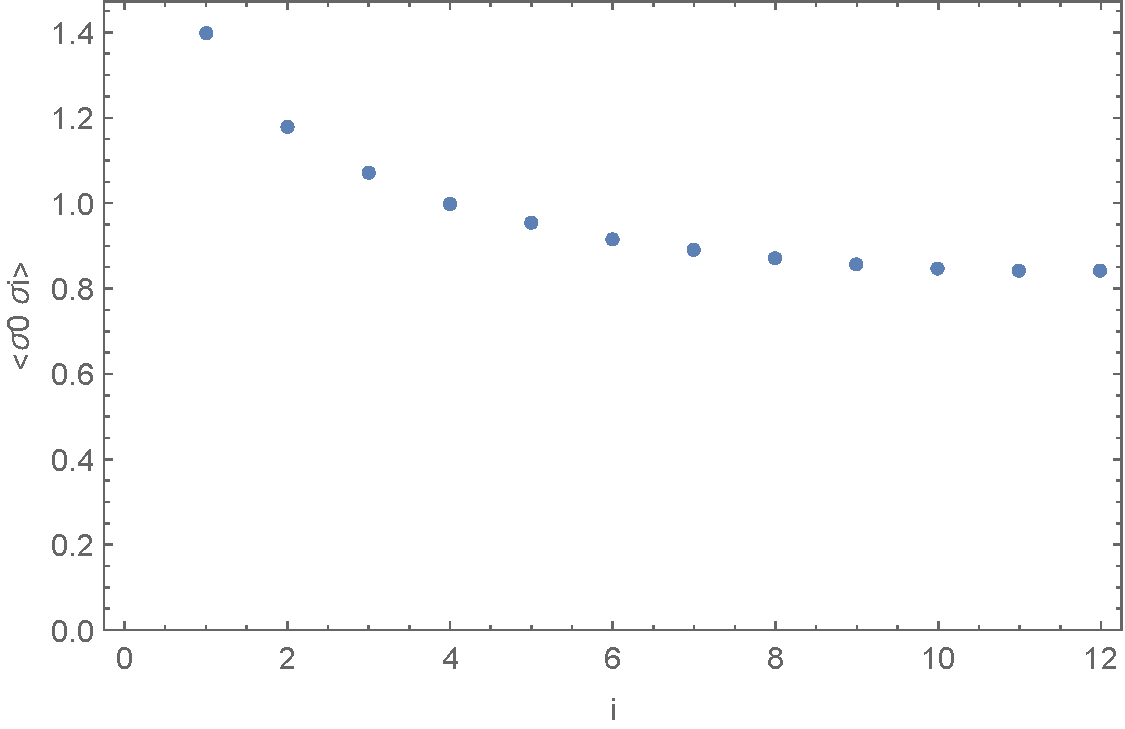
\includegraphics{fig-2pt-function.pdf}}
	\caption{\label{fig:ideal}CFT prediction for 2pt function at $N = 24$, Eq.
		\eqref{2ptideal}. }
\end{figure}

Prediction \eqref{2ptideal} is idealized because we can't find a microscopic
operator $s_i$ which exacty equals the CFT operator $\sigma (\phi_i)$. The
best we can hope for is a relation
\begin{equation}
	s_i = \sigma (\phi_i) + \ldots
\end{equation}
where {\ldots} stands for CFT operators of higher scaling dimension than
$\sigma$.

To find an appropriate operator $s_i$, let us start with $Z_i$, the simplest
microscopic operator diagonal in the $n_i$ basis. We can expand $Z_i$ in a sum
of $\mathbb{Z}_2$-even and $\mathbb{Z}_2$-odd CFT operators, as follows:
\begin{equation}
	Z_i = (- 1)^i \sum_{\mathbb{Z}_2 \text{-odd } \mathcal{O}} c_{\mathcal{O} }
	\mathcal{O}  (\phi_i) + \sum_{\mathbb{Z}_2 \text{-even } \mathcal{O}}
	c_{\mathcal{O}} \mathcal{O} (\phi_i)
\end{equation}


In the considered lattice model, lattice translation by one site maps to the
$\mathbb{Z}_2$ transformation of the CFT. This explains factor $(- 1)^i$ in
front of the sum over $\mathbb{Z}_2$-odd $\mathcal{O}$.

The first $\mathbb{Z}_2$-odd CFT operator is $\sigma$ that we are after, and
the first $\mathbb{Z}_2$-even CFT operator is the identity, which can be
subtracted by subtracting the vev of $Z_i$. Thus we identify the microscopic
operator: {\color{red}{REF}}
\begin{equation}
	s_i = (- 1)^i (Z_i - \langle Z_i \rangle) .
\end{equation}
We then have that $s_i = c_{\sigma} \sigma (\phi_i)$ plus corrections of
higher scaling dimension:
\begin{equation}
	s_i = c_{\sigma} \sigma (\phi_i) {+ c_{\partial_{\phi}^2 \sigma}} 
	\partial_{\phi}^2 \sigma (\phi_i) + (- 1)^i c_{\varepsilon} \varepsilon
	(\phi_i) + \ldots \label{sicorr}
\end{equation}
where we kept in the r.h.s. the corrections from two lowest $\mathbb{Z}_2$-odd
and $\mathbb{Z}_2$-even operators. This is all which can be said in general,
and in particular for point P1. For point P3, because of onsite $\mathbb{Z}_2$
symmetry, we have simplifications. All $\mathbb{Z}_2$-even operators have
$c_{\mathcal{O}} = 0$. Thus $\langle Z_i \rangle = 0$ so that the expression
for $s_i$ simplifies. Also $c_{\varepsilon} = 0$ so that $\varepsilon
(\phi_i)$ drops out from the correction term in \eqref{sicorr}.

Both for P1 and P3, since correction terms in \eqref{sicorr} have higher
scaling dimension than the leading term, we expect that the idealized
prediction \eqref{2ptideal} will hold at sufficiently large distances $| i - j
| \gg 1$. But at how large distances this holds depends a bit on luck - on how
large coefficients $c_{\mathcal{O}}$ of the correction term are with respect
to $c_{\sigma}$.

We pass on to simulations. We numerically compute the ground state
wavefunction for points P1 and P3. The ground state belongs to the
translationally invariant, spatial parity invariant subspace of the full
Hilbert space, which for $N = 24$ has dimension $352, 698$. Thus for $N = 24$
we can use exact diagonalization. This will be important for the optimization
of adiabatic evolution in Section \ref{sec:fidelity}.

We the compute the 2pt function $\langle s_i s_j \rangle$ which by the
symmetries of the problem is translationally and spatial parity invariant,
i.e. depends only on $| i - j |$. The result is shown in Fig.
\ref{fig:2pt-sim}, divided by the CFT prediction \eqref{2ptideal}. We see that
the ratios rapidly asymptote to a constant for both points P1 and P3. The
curves do show deviation from a constant at small $| i - j |$. These
deviations are due to the correction terms in \eqref{sicorr}. We see that for
point P3, where the correction term $(- 1)^i c_{\varepsilon} \varepsilon
(\phi_i)$ is absent, the approach to a constant is smoother and is monotonic.

\begin{figure}[h]\centering
	\resizebox{1\columnwidth}{!}{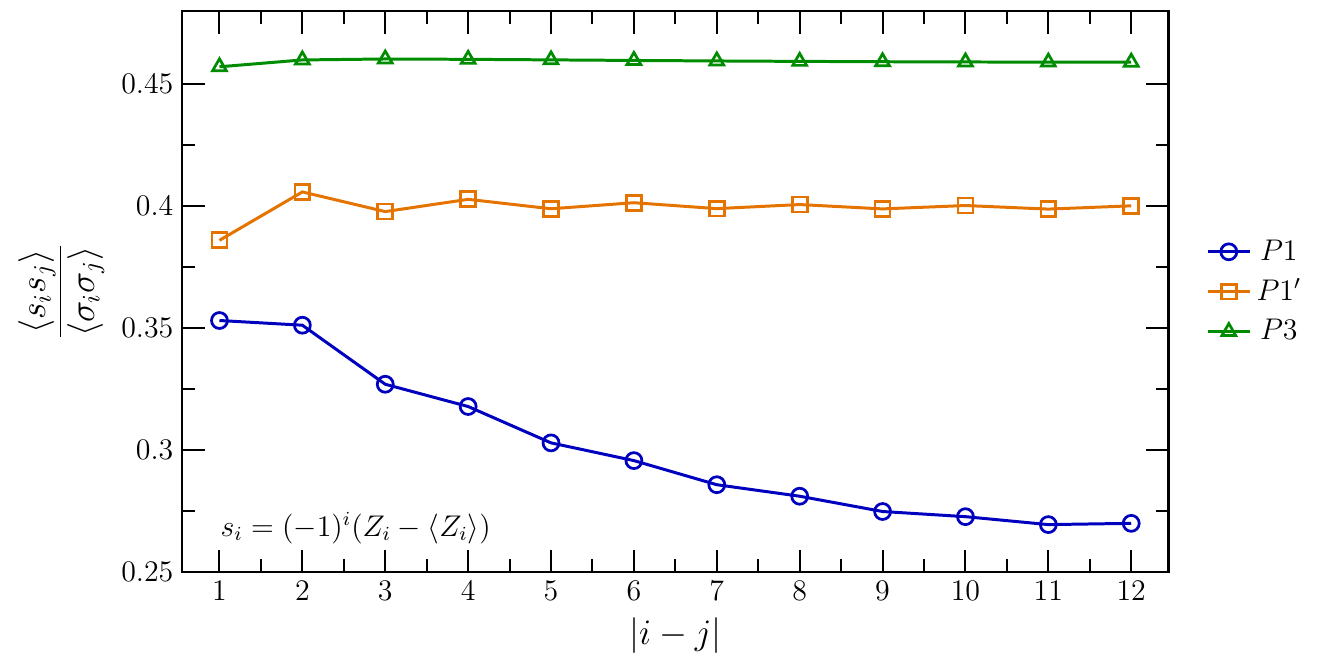
\includegraphics{fig-2pt-sim.png}}
	\caption{\label{fig:2pt-sim}2pt function simulations. {\color{red}{Remove
				P1, rename P1' as P1}}}
\end{figure}

Previously, numerical simulations of 2pt functions of the Rydberg spin chain
were discussed inin {\cite{Slagle:2021ene}}, focussing on the strong Rydberg
blockade regime where FSS effective Hamiltonian is applicable, and using the
same microscopic operator $s_i$, up to rescaling. There, oscillations in the
2pt function due to admixture of $(- 1)^j \epsilon (\phi)$ were also observed.

\subsection{Estimation of needed sample size}

\label{sec:sample}We learned in the previous section that the critical 2pt
function for relatively short chains of Rydberg atoms ($N = 24$) asymptotes to
its CFT form at distances order 1. In this section we will discuss how many
times one has to repeat the experiment to measure this 2pt function.

Consider the Hilbert space basis consisting of states $|n_0, \ldots, n_{N - 1}
\rangle$ where each $n_i = 0, 1$. We can expand the ground state in this
basis:
\begin{equation}
	| 0 \rangle = \sum_{n_i = 0, 1} a_{n_0, \ldots, n_{L - 1}} |n_0, \ldots,
	n_{L - 1} \rangle .
\end{equation}
In the experiment we will not have access to the full ground state
wavefunction itself but to {{\em collapsed states\/}} $\Psi_m$, $m = 1,
\ldots, M$, where $M$ is the number of times we repeated the experiment. Each
$\Psi_m$ is one of the basis states $|n_0, \ldots, n_{L - 1} \rangle$ and they
will appear in the experiment according to the Born rule, i.e. probability to
observe a collapsed state $|n_0, \ldots, n_{L - 1} \rangle$ equals $|a_{n_0,
	\ldots, n_{L - 1}} |^2$.

Any observable which is a function of $n_i$'s can be obtained experimentally
averaging over a sufficiently large number of collapsed states. The 2pt
function plotted in Fig.~\ref{fig:2pt-sim} is such an observable. How many
collapsed states is needed for a good signal-to-noise ratio? I.e.~how many
times $M$ shall we have to repeat the experiment? To answer this question, we
need to study the {{\em variance\/}} of our observable.

The variance of any observable $\mathcal{O}$ can be computed from the expected
value of $\mathcal{O}^2$.

Here we will not compute the variance but will estimate it, using a method
which is more direct and closer to the experiment. First, we compute the
ground state for $N = 24$ using exact diagonalization, working in the subspace
of translation and parity-invariant states, each of which is a finite linear
combination of \ the basis states $|n_0, \ldots, n_{L - 1} \rangle$. We then
sample the ground state, i.e. generate a sequence of random collapsed states
(``snapshots'') $|n_0, \ldots, n_{L - 1} \rangle$ distributed according to the
Born rule. (This is done in two steps: we first get a random translation and
parity-invariant state, and then one of its constituents.) This allows us to
simulate the experimental process directly. Statistical errors will go down as
$\Sigma / \sqrt{M}$, where $M$ is the number of snapshots, with $\Sigma$
estimated from the ``exact diagonalization data''.\footnote{For sufficiently
	large $N$, ED will become unfeasable and one will have to switch to the DMRG
	algorithm {\cite{White1992,Schollwock2011}}. This produces the wavefunction as
	a matrix product state (MPS). Interestingly, MPS representation also allows
	for quick sampling, using the {\texttt{sample()}} function of the
	{\texttt{iTensor.jl}} package.}

In our calculation we picked $M = 2 \times 10^3$. For each of $M$ collected
collapsed states $\Psi_m$ we measure the 2pt function $\langle s_0 s_j
\rangle$ as a function of $j$ (averaging over translations):
\begin{equation}
	\label{sample} X_m (j) = \frac{1}{N}  \sum_{i = 0}^{N - 1} \langle \Psi_m
	|s_i s_{i + j} | \Psi_m \rangle .
\end{equation}
For a fixed $j,$ $\{ X_m (j) \}_{m = 1}^M$ is a set of $M$ independent
identically distributed random variables, whose mean $\overline{X (j)}$ is the
ground-state 2pt function $\langle 0| s_0 s_j |0 \rangle$. The mean and the
standard deviation $\Sigma$ are estimated by the standard formulas
{\color{red}{REF}}
\begin{equation}
	\overline{X (j)}_{est} = \frac{1}{M}  \sum_m X_m (j), \qquad \Sigma
	(j)^2_{est} = \frac{1}{M - 1}  \sum_m (X_m (j) - \overline{X (j)})^2
	\hspace{0.17em} .
\end{equation}
By the central limit theorem, for $M \to \infty$, the sample mean $\overline{X
	(j)}_{est}$ has a gaussian distribution with variance $(\Sigma (j) /
\sqrt{M})^2$ around the true mean. We therefore obtain an estimation of the
2pt correlator, including one standard deviation error bars, as
\begin{equation}
	\langle s_0 s_j \rangle_{est} = \overline{X (j)}_{est} \pm
	\frac{1}{\sqrt{M}}  \sqrt{\Sigma (j)^2_{est}} . \label{eq:conf}
\end{equation}
In Fig.~\ref{ZZ2ptsample} we show the result of applying this procedure to the
critical 2pt function for $N = 24$ and $M = 2 \times 10^3$ samples. We see
that the statistical error is only a few percent.

\begin{figure}[h]\centering
	\begin{center}
		\resizebox{0.6\columnwidth}{!}{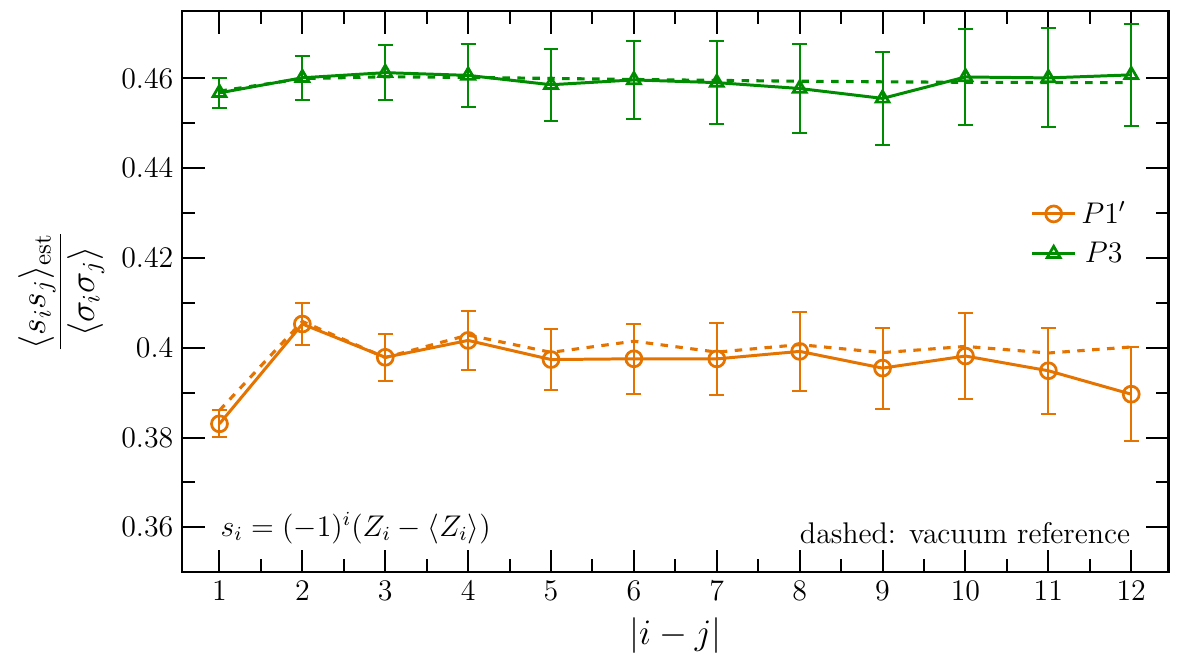
\includegraphics{fig-sampling.png}}\label{ZZ2ptsample}
	\end{center}
	\caption{Estimating the critical 2pt function on the ring of $N = 24$ atoms
		from independent snapshots, for points P1 and P3. {\color{red}{Rename P1' as
				P1}}}
\end{figure}

\subsection{Ground state preparation}

\label{sec:fidelity}In the previous sections, we have seen that if the
critical ground state can be obtained, then the critical 2pt function can be
measured, with good statistics achievable with $O (10^3)$ repetitions.

Experimentally, one realizes the critical ground state via adiabatic
evolution.

Let us follow the same protocol as in {\cite{Fang:2024uyf}}, start evolution
with $\Delta' < 0$, $\Omega' = 0$ in the state $| 00 \ldots 0 \rangle$ (i.e.
all atoms in the ground state). This state is in the disordered phase ground
state for $\Delta' < 0$, $\Omega' = 0$. One then picks the evolution
dependences (called ``ramp profile'') $\Omega' (t), \Delta' (t)$ which ends on
the Ising critical line. By the adiabatic theorem, if evolution is
sufficiently slow, the end state will approximate the critical ground state in
finite volume. However, for experimental reasons, evolution cannot be
arbitrarily slow. One wants it to be sufficiently slow so that good ground
state fidelity is achieved, yet as fast as possible, to reduce decoherence
effects to be discussed in Section \ref{sec:decoherence}.

For optimization purposes, we will fix a path in the $(\Omega', \Delta')$
plane and we will vary the local rate of change and the total evolution time.
For definiteness, we fix a two-segment path for point P1 and a three-segment
path for P3, see Fig. \ref{fig:evolution}.

The first path is precisely the one used in {\cite{Fang:2024uyf}}, where
total evolution time was $t_f = 7 \mu \text{s}$ split as $2 \mu \text{s} + 5
\mu \text{s}$ between the two segments, and the ramp profile $\Omega' (t),
\Delta' (t)$ shown in Fig. \ref{fig:yao-ramp}. In particular, linearly growing
$\Omega' (t)$ was chosen during the first secment, while during the second
segment $\Delta' (t)$ was chosen as a rational function with decreasing first
derivative. This was motivated by the locally adiabatic approximation
{\cite{Roland:2001imn}}, which parametrizes evolution in terms of the gap
between the ground state and the first excited state. Gap closes at the
critical point in the theremodynamic limit, while remains finite at finite
$N$.

\begin{figure}[h]\centering
	\resizebox{0.6\columnwidth}{!}{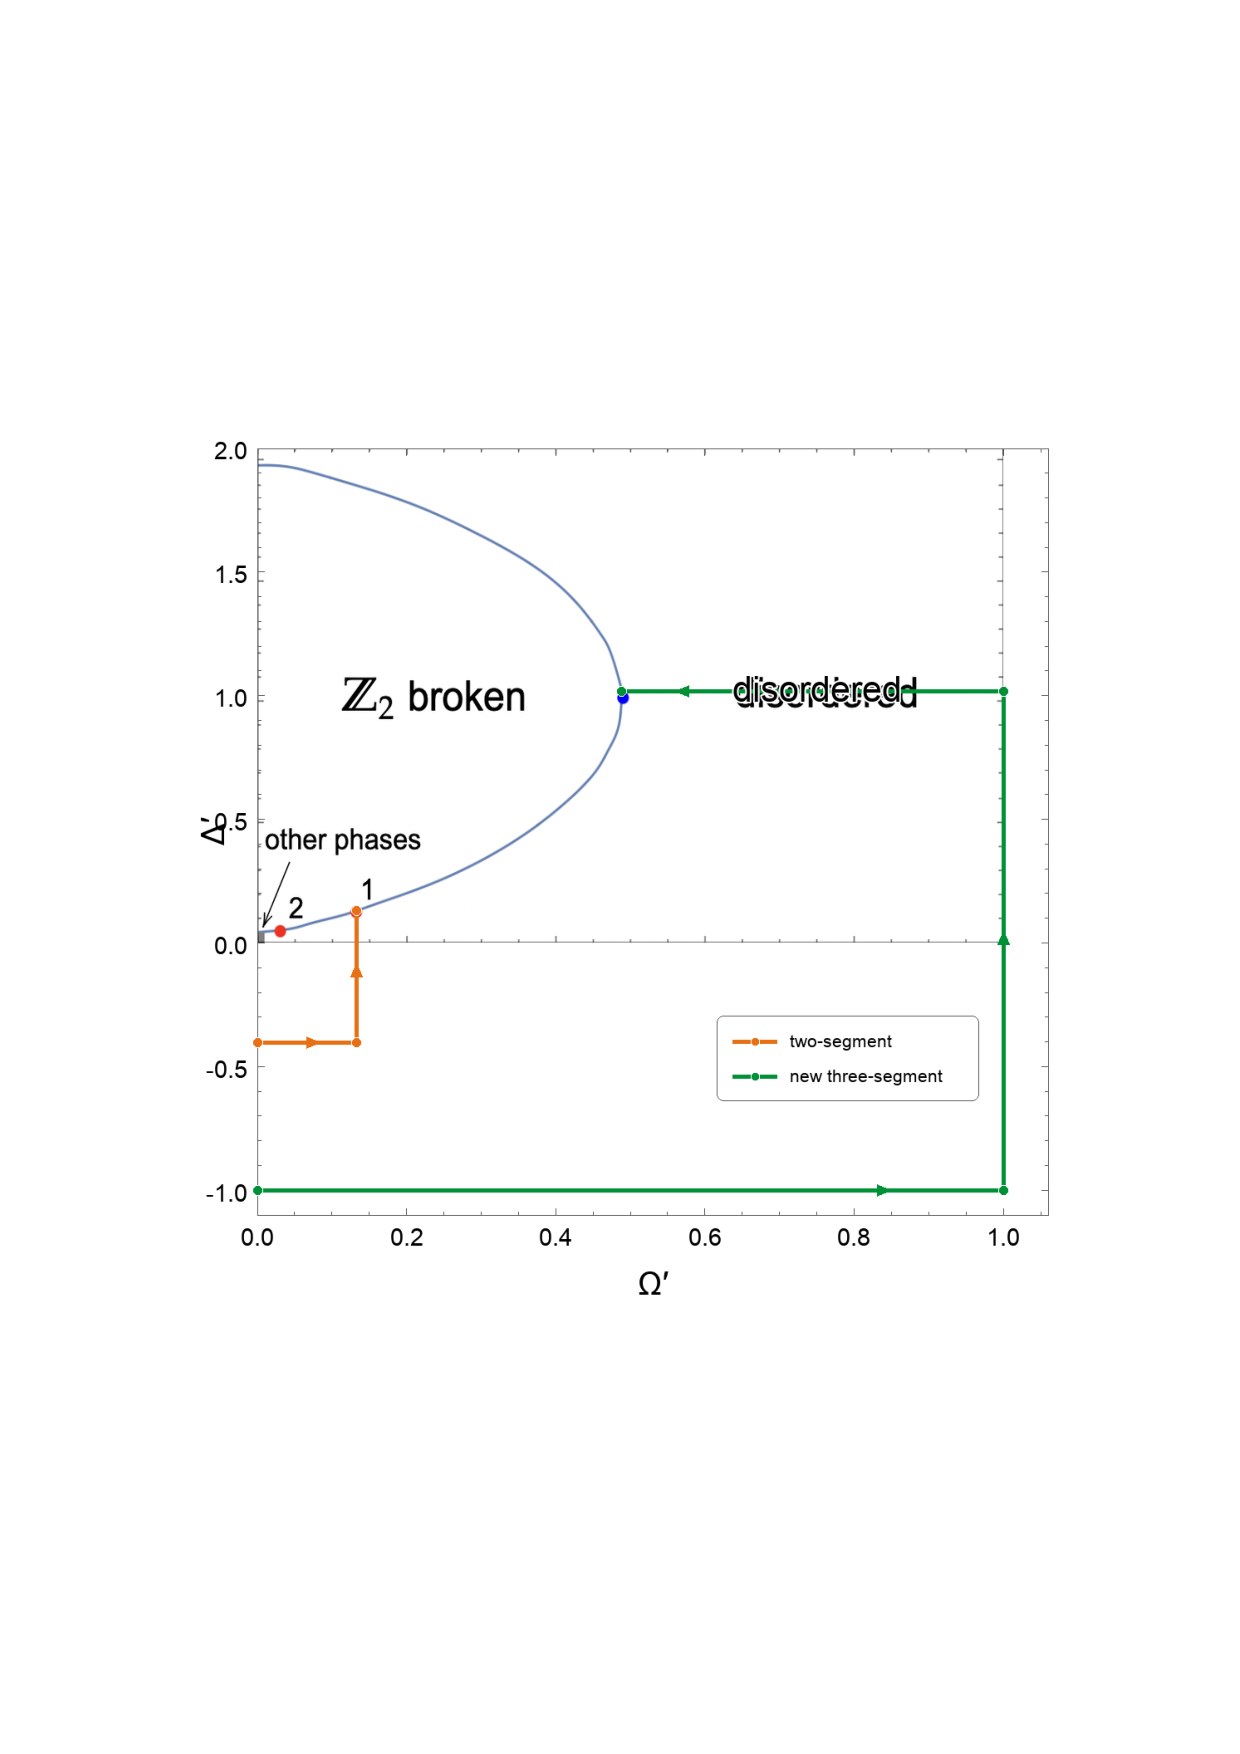
\includegraphics{fig-evolution.pdf}}
	\caption{\label{fig:evolution}Adiabatic evolution paths.}
\end{figure}

$N = 24$ is small enough so that full quantum mechanical evolution
\begin{equation}
	i \hbar \dot{\psi} (t) = U \hat{H} (\Omega' (t), \Delta' (t)) \psi
\end{equation}
can be solved numerically for any chosen ramp profile; see Appendix
\ref{sec:validation}. This evolution happens within the same translation and
spatial-parity invariant $352, 698$-dimensional subspace of the Hilbert space
to which the ground state belongs. We fix $U = \hbar \times
75.69\ensuremath{\operatorname{MHz}}$ as in {\cite{Fang:2024uyf}}. We can
expand the wave function $\psi (t)$ in eigenstates of the Hamiltonian at time
$t$:
\begin{equation}
	\psi (t) = \sum_{n = 0}^{\infty} c_n (t)  | n (t)  \rangle .
\end{equation}
We refer to $| c_0 (t_f) |$ as the ramp fidelity. The closer it is to 1, the
better the final state approximates the critical ground state. For the ramp in
{\cite{Fang:2024uyf}}, we find fidelity ??, see Table

\begin{table}[h]
	\begin{tabular}{lllllll}
		&   & $t_f, \mu \text{s}$ & $| c_0 (t_f) |$ & $| c_1 (t_f) |$ & $| c_2
		(t_f) |$ & $\left( 1 - \sum_{n = 0}^2 | c_n (t_f) |^2 \right)^{1 / 2}$\\
		ramps to P1: & {\cite{Fang:2024uyf}}, Fig. \ref{fig:yao-ramp} & 7 &  &  & 
		& \\
		&  & 2 &  &  &  & \\
		&  & 1.5 &  &  &  & \\
		ramps to P3: &  & ? &  &  &  & \\
		&  & ? &  &  &  & 
	\end{tabular}
	\caption{\label{tab:ramps}Ramp fidelities.}
\end{table}

As we will now describe, for $N = 24$, with modest computational resources one
can optimize ramp profiles, achieving better ground state fidelities than in
{\cite{Fang:2024uyf}} with several times shorter evolution times for point P1,
and even shorter times for point P3.

The computation is split into two phases - optimization and validation. In the
optimization stage, the model is reduced to a 20-dimensional subspace of the
20 lowest-energy states (locally for each $\Omega', \Delta'$). This reduced
model is small enough so that optimization can be performed. In the validation
stage, one checks fidelities via quantum mechanical evolution in the full
$352, 698$-dimensional subspace. See Appendix \ref{sec:optim} for details.

\subsection{Decoherence effects}\label{sec:decoherence}

For $a = 10 \mu$\text{{\rmfamily{m}}}, $U / \hbar = 0.86 \mathrm{rad} \cdot
\mu \mathrm{s}^{- 1}$ we get $v \approx 27 m / s$.

Tip advantage: For the same $U$, the energy gap is about factor 3 higher at
the tip than at the Yau point.

Important things to keep in mind:

Consider idealized situation when centers of potential wells have no
uncertainty, but there is uncertainty in the positions of the atoms due to the
size of the wavefunction $\Delta x$ and the size of the momentum $\Delta p
\sim \hbar / (\Delta x)$. (in practice a bit more because of nonzero
temperature)

Then the full uncertainty after time $\tau$ is
\begin{equation}
	\Delta x_{full} = \Delta x + \frac{\hbar}{\Delta x} M^{- 1} \tau
\end{equation}
where $M$ is the mass of an atom. (Double-check - influence of van der Waals
interaction on the atomic motion)

We want $\Delta x_{full} / a \ll 1$, which limits $\Delta x$ and $\tau$ from
above.

It makes sense to set $\tau$ so that $\Delta x = \epsilon a$,
$\frac{\hbar}{\Delta x} M^{- 1} \tau = \epsilon a$, so $\tau = a^2 \epsilon^2
\hbar^{- 1} M$

We can increase $a$, but then $U = C_6 / a^6$ decreases and hence the energy
gap decreases.

We want $E_{gap} \tau \gg \hbar$.

We have $E_{gap} \tau \hbar^{- 1} = 3.12 C_6 / a^6 N^{- 1} a^2 \epsilon^2
\hbar^{- 2} M = 3.12 C_6 / a^4 N^{- 1} \epsilon^2 \hbar^{- 2} M$

We see that, for fixed $\epsilon$, we want to take $a$ as small as possible,
i.e. $\Delta x$ as small as possible.

Thus the limiting factor for adiabaticity will be $\Delta x$. So we can
rewrite the previous equation as

$E_{gap} \tau \hbar^{- 1} = 3.12 C_6 / (\Delta x)^4 N^{- 1} \epsilon^{- 2}
\hbar^{- 2} M$

Parameters: Rubidium $n = 60$ level Pasqual: $C_6 / \hbar = 865723 (\mu s)^{-
	1}  (\mu m)^6$, $\Delta x = 0.1 \mu m$ (optimistic), $M_{Rb} = 87$

Local adiabatic evolution: {\cite{Richerme:2013hbx}} important is the lowest
$\mathbb{Z_2}$ state.

Norman Yao: ramp time 5 $\mu s$.

Summary: mention trap parameters for various experiments, and various $C_6$,
various evolution times

Describe Norman Yao setup in detail

{\color{red}{stopped here, working below}}

The experimentally accessible parameter space is, roughly, {\cite[Tab.
	1]{noise-note}}

\begin{align}
	\Omega' \in [0, 2], \quad \Delta' \in [- 10, 20] . 
\end{align}

Plan: investigate the $\mathbb{Z}_2$-even energy gap landscape.

{\color{red}{JR:On the phase diagram of the Rydberg atom, at generic 2nd order
		transition point, the $\mathbf{Z}_2$ symmetry is given by the translation.
		However, in the special point we discussed, the model becomes literally the
		AFM Ising model, we can easily get the free boundary condition. We should
		probably mention this later}}

\subsection{Prospects for the measurement: summary}\label{sec:prospects}

\section{Conclusions}\label{sec:concl}

\text{{\bfseries{Acknowledgements}}}

We thank colleagues at the Institut d'Optique, Ecole Polytechnique (Antoine
Browaeys, Thierry Lahaye, David Clement, Thomas Chalopin), PASQUAL (Guillaume
Villaret, Adrien Signoles, Alexander Dauphin), and Institute for Advanced
Study, Tsinghua University (Wenlan Chen, Yingfei Gu, Chengshu Li) for
discussions of cold atom experiments. SR also thanks Hans Peter B{\"u}chler
and Enrico Rinaldi for discussions. SR is partially supported by the Simons
Collaboration on the Probabilistic Paths to Quantum Field Theory (award
SFI-MPS-PP-00012621-16).

\section*{Data availability statement}

The DMRG code ??? is available from the authors upon request.

\appendix

\section{Some details about the experiment of Ref. {\cite{Fang:2024uyf}}}

Ref. {\cite{Fang:2024uyf}} measured 1D and 2D arrays of Rydberg atoms tuned to
the quantum critical point in the Ising universalty class. We will report here
parameters of their experiments, focussing on 1D case of relevance for this
paper.

The Hamiltonian of Ref. {\cite{Fang:2024uyf}} is precisely \eqref{eq:model}
with $N = 24$ atoms on a circle (they also studied $N = 40$). To reach the
critical state they evolve $\Delta, \Omega$ as in Fig. \ref{fig:yao-ramp}.
They report the following endpoint parameters:
\begin{equation}
	\Omega  / 2 \pi = 1.6\ensuremath{\operatorname{MHz}}, \quad \Delta / \Omega 
	= 0.97 (5), \quad R_b / a \approx 1.4,
\end{equation}
where $R_b = (C_6 / \hbar \Omega)^{1 / 6}$ is the blockade radius (they don't
report the error on $R_b / a$). Combining these we compute:
\begin{equation}
	U = C_6 / a^6 \approx \hbar \times 2 \pi 1.6 1.4^4
	\ensuremath{\operatorname{MHz}}= \hbar \times
	75.69\ensuremath{\operatorname{MHz}},
\end{equation}
\begin{equation}
	\Omega' = \hbar \Omega / U \approx 1 / 1.4^6 \approx 0.133 .
\end{equation}
The point P1 in Table \ref{tab:params} has $\Delta' / \Omega' = 1.03$, at the
upper end of the range $\Delta / \Omega  = 0.97 (5)$ from Ref.
{\cite{Fang:2024uyf}}.

\begin{figure}[h]\centering
	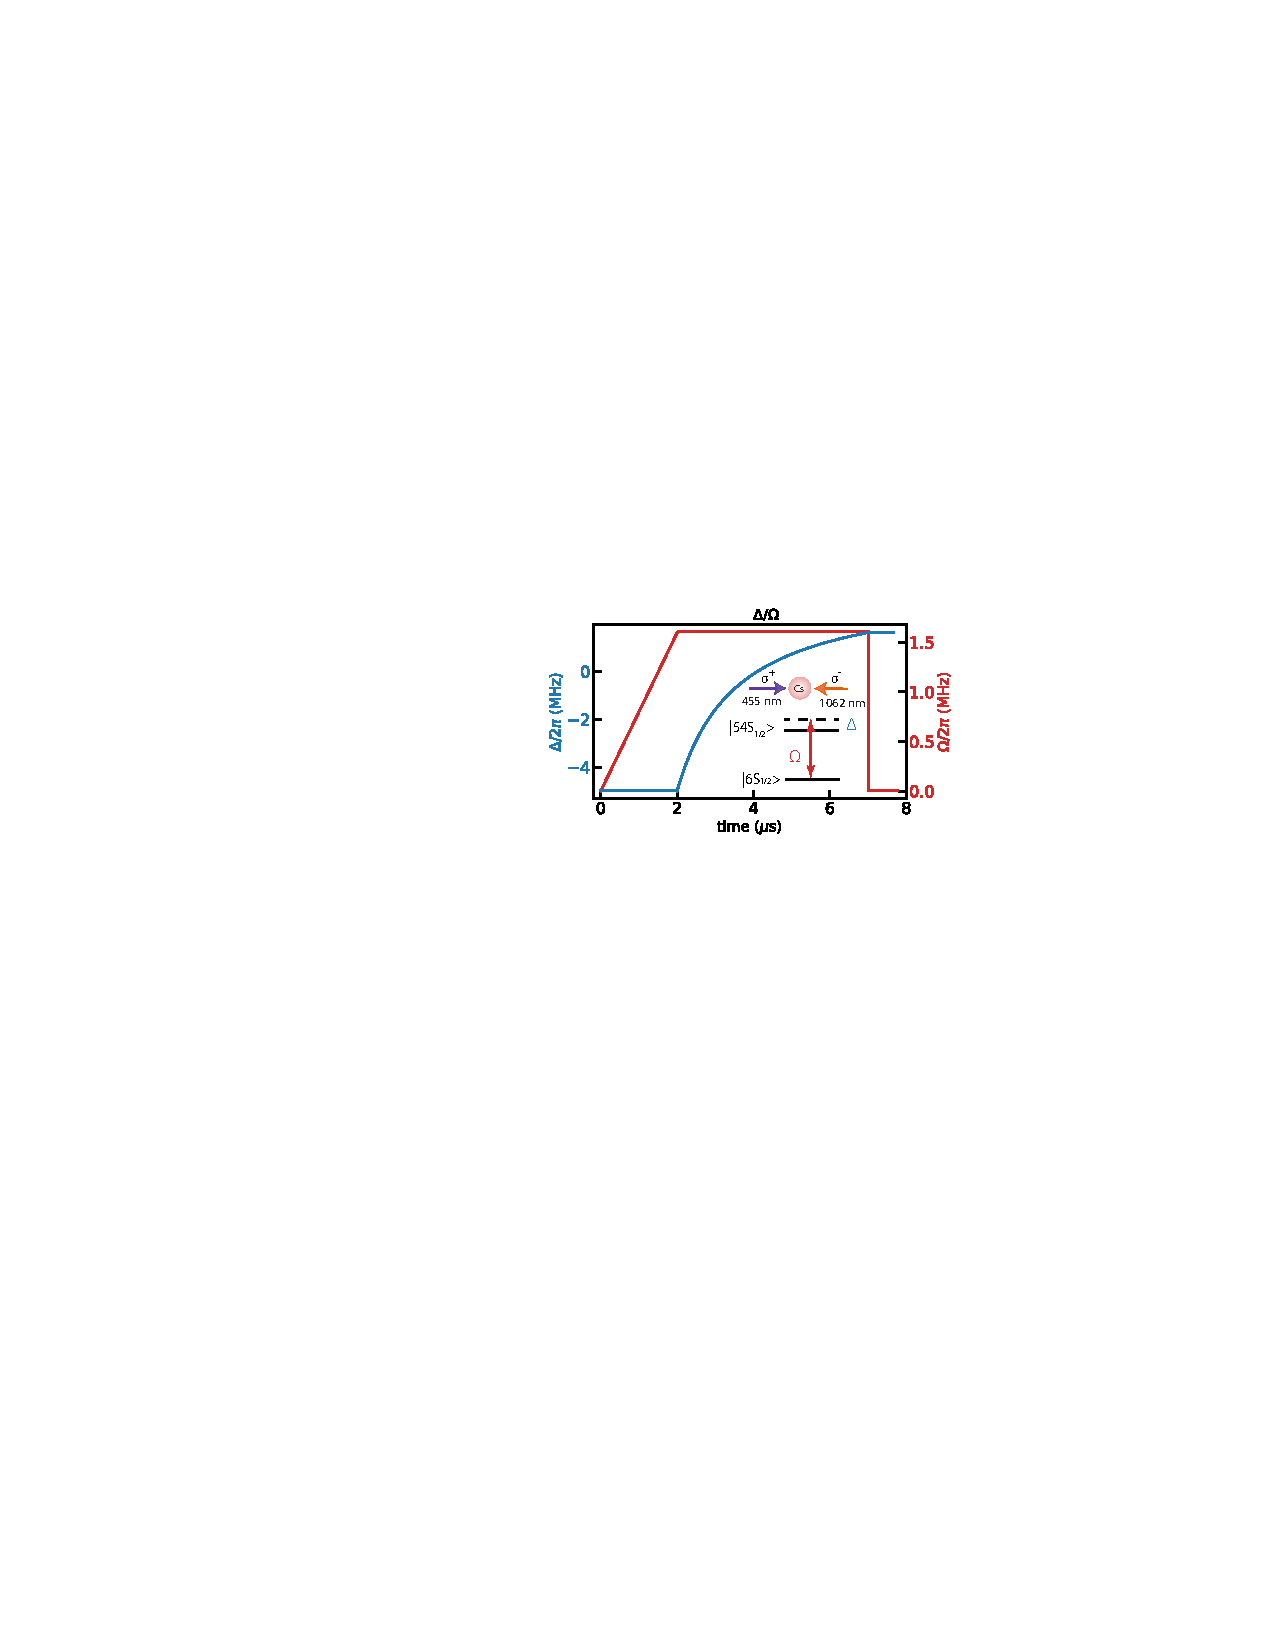
\includegraphics{fig-Yao-ramp.pdf}
	\caption{\label{fig:yao-ramp}Evolution $\Delta (t)$ and $\Omega (t)$ for
		preparing the critical state in {\cite{Fang:2024uyf}}, Fig. 1C. }
\end{figure}

Ref. {\cite{Fang:2024uyf}} used the experimental definition of the critical
point, as the location of the maximum of susceptibility $\partial \langle n
\rangle / \partial \Delta$ for sufficiently slow sweeps. They note that this
also coincides with the excitation gap minimum. For measuring the 2pt function
a better theoretical definition of the critical point is where the properties
of the system are described by the CFT Hamiltonian. This may differ by $1 / N$
effects from the definitions used in Ref. {\cite{Fang:2024uyf}}. Our
simulations show the point P1 with $\Delta' / \Omega' = 1.03$ gives the 2pt
function consistent with CFT, while $\Delta' / \Omega' = 0.97$ would give a
2pt function decaying faster than CFT (thus in the disordered phase), with
$\sim 20\%$ suppression at the largest separation.

The 2pt function measured in {\cite{Fang:2024uyf}}, Fig. 2F, was fitted by
them by the curve
\begin{equation}
	\langle s_0 s_j \rangle \propto \delta^{- 1 / 4}_j \exp (- \delta_j / \xi ),
	\quad \delta_j = a \frac{N}{\pi} \sin \left( \frac{\pi j}{N} \right),
\end{equation}
and $\xi / a = 13.2^{+ 5.7}_{- 3.6}$ is the correlation length, attributed to
decoherence. The central $\xi$ value corresponds to about 50\% suppression of
the correlator at the largest separation w.r.t. the CFT value.

\section{Ramp profile optimization}\label{sec:optim}

Optimization algorithm includes optimization in reduced 20-dimensional
subspace and validation in full $352, 698$-dimensional subspace. We discuss
validation first.

\subsection{Validation}\label{sec:validation}

\subsection{Optimization within reduced subspace}\label{sec:reduced}

Optimization stage:

The path is discretized. A few hundred discretization points works well. For
each discretization point $(\Omega', \Delta')$, Hamiltonian is diagonalized
and the lowest $K$ states are kept ($K = 20$ works well). One makes sure that
this basis varies continuously with $\Omega', \Delta'$ \ The wavefunction is
thus approximated by its projection onto the subspace of the 20 lowest-energy
states (locally for each $\Omega', \Delta'$), and the Hamiltonian is a $20
\times 20$ matrix, depending on $\Omega', \Delta'$.



	
\bibliographystyle{utphys}
\small
\setlength{\bibsep}{2pt}
\bibliography{reference.bib}


\end{document}
